% Escolha: Portugues ou Ingles ou Espanhol.
% Para a versão final do texto, após a defesa, acrescente Final:

\documentclass[Ingles,Final]{ic-tese-v3}
%\documentclass[Portugues,Final]{ic-tese-v3}

\usepackage[latin1,utf8]{inputenc}
%\usepackage{todonotes}
\usepackage{hyperref}
\usepackage{amsmath}
\usepackage{amssymb}
\usepackage{amsfonts}
\usepackage{multirow}
\usepackage{multicol}
\usepackage{graphicx}
\usepackage{float}
\usepackage{caption}
\usepackage[font=footnotesize]{subcaption}
\usepackage{array}
\usepackage{color}
\usepackage{colortbl}
\usepackage[table]{xcolor}
\usepackage{ntheorem}
\usepackage{IEEEtrantools}
%\usepackage[color=blue!20]{todonotes}
%\usepackage{hyperref}
\usepackage{url}
%\usepackage{subfigure}
\usepackage{booktabs}
\usepackage{tikz}
\usepackage{flushend}
%\usepackage{cite}
% My Table

\colorlet{tableheadcolor}{gray!25} % Table header colour = 25% gray
\colorlet{tablerowcolor}{gray!10} % Table row separator colour = 10% gray

\newcommand{\headcol}{\rowcolor{tableheadcolor}} %
\newcommand{\rowcol}{\rowcolor{tablerowcolor}} %

% Command \topline consists of a (slightly modified) \toprule followed by a \heavyrule rule of colour tableheadcolor (hence, 2 separate rules)
\newcommand{\topline}{\arrayrulecolor{black}\specialrule{0.1em}{\abovetopsep}{0pt}%
    \arrayrulecolor{tableheadcolor}\specialrule{\belowrulesep}{0pt}{0pt}%
    \arrayrulecolor{black}}

% Command \midline consists of 3 rules (top colour tableheadcolor, middle colour black, bottom colour white)
\newcommand{\midline}{\arrayrulecolor{tableheadcolor}\specialrule{\aboverulesep}{0pt}{0pt}%
    \arrayrulecolor{black}\specialrule{\lightrulewidth}{0pt}{0pt}%
    \arrayrulecolor{white}\specialrule{\belowrulesep}{0pt}{0pt}%
    \arrayrulecolor{black}\hline}

% Command \rowmidlinecw consists of 3 rules (top colour tablerowcolor, middle colour black, bottom colour white)
\newcommand{\rowmidlinecw}{\arrayrulecolor{tablerowcolor}\specialrule{\aboverulesep}{0pt}{0pt}%
    \arrayrulecolor{black}\specialrule{\lightrulewidth}{0pt}{0pt}%
    \arrayrulecolor{white}\specialrule{\belowrulesep}{0pt}{0pt}%
    \arrayrulecolor{black}}

% Command \rowmidlinewc consists of 3 rules (top colour white, middle colour black, bottom colour tablerowcolor)
\newcommand{\rowmidlinewc}{\arrayrulecolor{white}\specialrule{\aboverulesep}{0pt}{0pt}%
    \arrayrulecolor{black}\specialrule{\lightrulewidth}{0pt}{0pt}%
    \arrayrulecolor{tablerowcolor}\specialrule{\belowrulesep}{0pt}{0pt}%
    \arrayrulecolor{black}}

% Command \rowmidlinew consists of 1 white rule
\newcommand{\rowmidlinew}{\arrayrulecolor{white}\specialrule{\aboverulesep}{0pt}{0pt}%
    \arrayrulecolor{black}}

% Command \rowmidlinec consists of 1 tablerowcolor rule
\newcommand{\rowmidlinec}{\arrayrulecolor{tablerowcolor}\specialrule{\aboverulesep}{0pt}{0pt}%
    \arrayrulecolor{black}}

% Command \bottomline consists of 2 rules (top colour
\newcommand{\bottomline}{\arrayrulecolor{white}\specialrule{\aboverulesep}{0pt}{0pt}%
    \arrayrulecolor{black}\specialrule{\heavyrulewidth}{0pt}{\belowbottomsep}}%
\newcommand{\bottomlinec}{\arrayrulecolor{tablerowcolor}\specialrule{\aboverulesep}{0pt}{0pt}%
    \arrayrulecolor{black}\specialrule{\heavyrulewidth}{0pt}{\belowbottomsep}}%
\newcommand{\bottomlinehc}{\arrayrulecolor{tableheadcolor}\specialrule{\aboverulesep}{0pt}{0pt}%
    \arrayrulecolor{black}\specialrule{\heavyrulewidth}{0pt}{\belowbottomsep}}%

\newcommand*{\rulefillerh}{%
    \arrayrulecolor{tableheadcolor}% change to cell colour
    \specialrule{\heavyrulewidth}{0pt}{-\heavyrulewidth}% "invisible" rule
    \arrayrulecolor{black}% revert to regular line colour
}

\newcommand*{\rulefillerc}{%
    \arrayrulecolor{tablerowcolor}% change to cell colour
    \specialrule{\heavyrulewidth}{0pt}{-\heavyrulewidth}% "invisible" rule
    \arrayrulecolor{black}% revert to regular line colour
}

\let\mcol\multicolumn
\let\ml\multirow

\usepackage{pdflscape}
\usepackage{longtable}

\usepackage{listings}


%For float barrier
\usepackage{placeins}

%For citations
\usepackage[numbers,square,comma,]{natbib}
\usepackage{bibentry}
\usepackage{notoccite}


%Rotating things
\usepackage{rotating}

\definecolor{codegreen}{rgb}{0,0.6,0}
\definecolor{codegray}{rgb}{0.5,0.5,0.5}
\definecolor{codepurple}{rgb}{0.58,0,0.82}
\definecolor{backcolour}{rgb}{0.95,0.95,0.92}

\lstdefinestyle{fancyterminal}{
    backgroundcolor=\color{backcolour},   
    commentstyle=\color{codegreen},
    keywordstyle=\color{magenta},
    numberstyle=\tiny\color{codegray},
    stringstyle=\color{codepurple},
    basicstyle=\scriptsize\ttfamily,
    breakatwhitespace=false,         
    breaklines=true,                 
    captionpos=b,                    
    keepspaces=true,
%    numbers=left,                    
    numbersep=5pt,                  
    showspaces=false,                
    showstringspaces=false,
    showtabs=false,                  
    tabsize=2
}

\lstdefinestyle{terminal}
{
    backgroundcolor=\color{black},
    basicstyle=\scriptsize\color{white}\ttfamily
    commentstyle=\color{codegreen},
    keywordstyle=\color{magenta},
    numberstyle=\tiny\color{codegray},
    stringstyle=\color{codepurple},
    breakatwhitespace=false,         
    breaklines=true,                 
    captionpos=b,                    
    keepspaces=true,
%    numbers=left,                    
    numbersep=5pt,                  
    showspaces=false,                
    showstringspaces=false,
    showtabs=false,                  
    tabsize=2
}

%\lstset{style=mystyle}



% Example definitions.
% --------------------
\def\x{{\mathbf x}}
\def\L{{\cal L}}
\newcommand{\etal}[1]{#1~\textit{et~al.}}
%% My Table

\colorlet{tableheadcolor}{gray!25} % Table header colour = 25% gray
\colorlet{tablerowcolor}{gray!10} % Table row separator colour = 10% gray

\newcommand{\headcol}{\rowcolor{tableheadcolor}} %
\newcommand{\rowcol}{\rowcolor{tablerowcolor}} %

% Command \topline consists of a (slightly modified) \toprule followed by a \heavyrule rule of colour tableheadcolor (hence, 2 separate rules)
\newcommand{\topline}{\arrayrulecolor{black}\specialrule{0.1em}{\abovetopsep}{0pt}%
    \arrayrulecolor{tableheadcolor}\specialrule{\belowrulesep}{0pt}{0pt}%
    \arrayrulecolor{black}}

% Command \midline consists of 3 rules (top colour tableheadcolor, middle colour black, bottom colour white)
\newcommand{\midline}{\arrayrulecolor{tableheadcolor}\specialrule{\aboverulesep}{0pt}{0pt}%
    \arrayrulecolor{black}\specialrule{\lightrulewidth}{0pt}{0pt}%
    \arrayrulecolor{white}\specialrule{\belowrulesep}{0pt}{0pt}%
    \arrayrulecolor{black}\hline}

% Command \rowmidlinecw consists of 3 rules (top colour tablerowcolor, middle colour black, bottom colour white)
\newcommand{\rowmidlinecw}{\arrayrulecolor{tablerowcolor}\specialrule{\aboverulesep}{0pt}{0pt}%
    \arrayrulecolor{black}\specialrule{\lightrulewidth}{0pt}{0pt}%
    \arrayrulecolor{white}\specialrule{\belowrulesep}{0pt}{0pt}%
    \arrayrulecolor{black}}

% Command \rowmidlinewc consists of 3 rules (top colour white, middle colour black, bottom colour tablerowcolor)
\newcommand{\rowmidlinewc}{\arrayrulecolor{white}\specialrule{\aboverulesep}{0pt}{0pt}%
    \arrayrulecolor{black}\specialrule{\lightrulewidth}{0pt}{0pt}%
    \arrayrulecolor{tablerowcolor}\specialrule{\belowrulesep}{0pt}{0pt}%
    \arrayrulecolor{black}}

% Command \rowmidlinew consists of 1 white rule
\newcommand{\rowmidlinew}{\arrayrulecolor{white}\specialrule{\aboverulesep}{0pt}{0pt}%
    \arrayrulecolor{black}}

% Command \rowmidlinec consists of 1 tablerowcolor rule
\newcommand{\rowmidlinec}{\arrayrulecolor{tablerowcolor}\specialrule{\aboverulesep}{0pt}{0pt}%
    \arrayrulecolor{black}}

% Command \bottomline consists of 2 rules (top colour
\newcommand{\bottomline}{\arrayrulecolor{white}\specialrule{\aboverulesep}{0pt}{0pt}%
    \arrayrulecolor{black}\specialrule{\heavyrulewidth}{0pt}{\belowbottomsep}}%
\newcommand{\bottomlinec}{\arrayrulecolor{tablerowcolor}\specialrule{\aboverulesep}{0pt}{0pt}%
    \arrayrulecolor{black}\specialrule{\heavyrulewidth}{0pt}{\belowbottomsep}}%
\newcommand{\bottomlinehc}{\arrayrulecolor{tableheadcolor}\specialrule{\aboverulesep}{0pt}{0pt}%
    \arrayrulecolor{black}\specialrule{\heavyrulewidth}{0pt}{\belowbottomsep}}%

\newcommand*{\rulefillerh}{%
    \arrayrulecolor{tableheadcolor}% change to cell colour
    \specialrule{\heavyrulewidth}{0pt}{-\heavyrulewidth}% "invisible" rule
    \arrayrulecolor{black}% revert to regular line colour
}

\newcommand*{\rulefillerc}{%
    \arrayrulecolor{tablerowcolor}% change to cell colour
    \specialrule{\heavyrulewidth}{0pt}{-\heavyrulewidth}% "invisible" rule
    \arrayrulecolor{black}% revert to regular line colour
}

\let\mcol\multicolumn
\let\ml\multirow


\newcommand{\dataset}{{\cal D}}
\newcommand{\fracpartial}[2]{\frac{\partial #1}{\partial  #2}}
\newcommand{\expnumber}[2]{{#1}\times10^{#2}}
\newcommand{\highlight}[1]{\tikz[baseline]{\node[rounded corners,fill=green!25, anchor=base]{$\mathbf{#1}$}}}

\newcommand{\correcao}[1]{\textcolor{red}{#1}}


% Para acrescentar comentários ao PDF descomente:
\usepackage
%  [pdfauthor={nome do autor},
%   pdftitle={titulo},
%   pdfkeywords={palavra-chave, palavra-chave},
%   pdfproducer={Latex with hyperref},
%   pdfcreator={pdflatex}]
{hyperref}


\begin{document}

% Escolha entre autor ou autora:
\autor{Luís Gustavo Lorgus Decker}
%\autora{Nome da Autora}

% Sempre deve haver um título em português:
\titulo{Localização de Textos em Imagens de Cena Utilizando Redes Convolucionais Leves}

% Se a língua for o inglês ou o espanhol defina:
\title{Scene Text Localization Using Lightweight Convolutional Networks }

% Escolha entre orientador ou orientadora. Inclua os títulos acadêmicos:
\orientador{Prof. Dr. Ricardo da Silva Torres}
%\orientadora{Profa. Dra. Nome da Orientadora}

% Escolha entre coorientador ou coorientadora, se houver.  Inclua os títulos acadêmicos:
\coorientador{Dr. Allan da Silva Pinto}
%\coorientadora{Profa. Dra. Eng. Lic. Nome da Co-Orientadora}

% Escolha entre mestrado ou doutorado:
\mestrado
%\doutorado

% Se houve cotutela, defina:
%\cotutela{}

\datadadefesa{12}{03}{2020}

% Para a versão final defina:
\avaliadorA{Dr. Allan da Silva Pinto}{Instituto de Computação/UNICAMP}
\avaliadorB{Dr. Marcos Vinicius Mussel Cirne}{Instituto de Computação/UNICAMP}
\avaliadorC{Prof. Dr. Rodrigo Minetto}{DAINF/UFTPR}
%\avaliadorD{Prof. Dr. Quarto Avaliador}{Instituição do quarto avaliador}
%\avaliadorE{Prof. Dr. Quinto Avaliador}{Instituição do quinto avaliador}
%\avaliadorF{Prof. Dr. Sexto Avaliador}{Instituição do sexto avaliador}
%\avaliadorG{Prof. Dr. Sétimo Avaliador}{Instituição do sétimo avaliador}
%\avaliadorH{Prof. Dr. Oitavo Avaliador}{Instituição do oitavo avaliador}


% Para incluir a ficha catalográfica em PDF na versão final, descomente e ajuste:
\fichacatalografica{ficha_catalografica.pdf}


% Este comando deve ficar aqui:
\paginasiniciais


% Se houver dedicatória, descomente:
%\prefacesection{Dedicatória}
%A dedicatória deve ocupar uma única página.


% Se houver epígrafe, descomente e edite:
% \begin{epigrafe}
% {\it
% Vita brevis,\\
% ars longa,\\
% occasio praeceps,\\
% experimentum periculosum,\\
% iudicium difficile.}
%
% \hfill (Hippocrates)
% \end{epigrafe}


% Agradecimentos ou Acknowledgements ou Agradecimientos
\prefacesection{Acknowledgements}

%\todo[inline]{Are you planning to stretch this text?}

I would like to initially thank my advisor, Prof. Ricardo, and my co-advisor, Dr. Allan, for the valuable support on this journey; their comments, help, corrections, and incentives allowed me to develop this work.

I am especially grateful to Danelise, that without her love and her trust I would not have even taken the first steps in graduate school. Thank you so much for everything! I love you!

I thank my family, for all the strength and consideration throughout this period,  especially to my father Randolfo, who always believed in my potential and trusted in my endeavors!

I am grateful to my colleagues at the RECOD laboratory, especially to my SAMSUNG project colleagues. I also thank the Norwegian University of Science and Technology~(NTNU) for its support.

This work was partially funded by CNPq, S\~ao Paulo Research Foundation -- FAPESP (grants \#2014/12236-1, \#2015/24494-8, \#2016/50250-1, and \#2017/20945-0) and the FAPESP-Microsoft Virtual Institute (grants \#2013/50155-0 and \#2014/50715-9). This study was financed in part by the Coordena\c{c}\~{a}o de Aperfei\c{c}oamento de Pessoal de N\'{i}vel Superior - Brasil (CAPES) - Finance Code 001, and also by Samsung Eletr\^{o}nica da Amaz\^{o}nia Ltda., through the project ``Algoritmos para Detec\c{c}\~{a}o e Reconhecimento de Texto Multil\'{i}ngue (MLTSR)'', within the scope of the Informatics Law No. 8248/91.

% Sempre deve haver um resumo em português:
\begin{resumo}
%O resumo deve ter no máximo 500 palavras e deve ocupar uma única página.
Múltiplas frentes de pesquisa reportaram resultados altamente eficazes para o problema de detecção de texto, que consiste no desafio de detectar em uma imagem digital a posição de variados elementos textuais, como palavras e frases. Porém, muitas destas soluções são custosas, o que restringe o uso das mesmas em várias aplicações que dependem de dispositivos com capacidade computacional restrita, como relógios inteligentes e celulares. A localização de texto é um passo importante para várias aplicações importantes que podem ser executadas em ambientes embarcados, como tradução de textos e auxílio a deficientes visuais. Neste trabalho, tratamos deste problema a partir da investigação da possibilidade do uso de redes neurais eficientes usualmente empregadas para detecção de objetos. Propusemos a junção de duas arquiteturas leves, {\em MobilenetV2} e {\em Single Shot Detector (SSD)} em nossa proposta nomeada MobText para resolver o problema da detecção de texto. Resultados experimentais nos conjuntos de dados ICDAR'11 e ICDAR'13 demonstram que nossa proposta está associada a bons resultados tanto em termos de eficácia quanto de eficiência. Em especial, o método proposto obteve resultados estado-da-arte no conjunto de dados ICDAR'11, com {\em f-measure} de $96,09\%$, mantendo um tempo de processamento médio de $464 ms$ em um ambiente de processamento restritivo. Uma outra contribuição do trabalho consistiu na proposta de uma ferramenta para automatizar o processo de avaliação de métodos de detecção e reconhecimento de textos em imagens de cena.


%\todo[inline]{
%Um abstract é composto pelos seguintes elementos (\url{https://www.youtube.com/watch?v=e968B1PwIbs}):
%\begin{enumerate}
%     \item Contextualização;
%     \item Gap da área;
%     \item Objetivo do trabalho;
%     \item Metodo proposto;
%     \item Resultados;
%     \item Conclusão.
% \end{enumerate}
% Pontos a serem melhorados neste seu abstract:
% \begin{enumerate}
%     \item Contextualização: Precisa ser expandido.
%     Sugestão: Comece falando o que é detecção de texto e sua importância; e em qual grande %área seu trabalho se insere.
%     \item Gap da área: Está OK
%     \item Objetivo do trabalho: o que você está considerando para decidir se algo é %eficiente, ou não? Tempo? Memoria? FLOPS?
%     \item Método proposto: Está OK;
%     \item Resultados: Mostre um resultado relacionado a eficiencia também;
%     \item Conclusão: Escreva um ou dois parágrafos sobre as principais conclusões do seu %trabalho.
% \end{enumerate}
%}
%\todo{Linkar, traduzir e extender o abstract do artigo}
\end{resumo}


% Sempre deve haver um abstract:
\begin{abstract}
Multiple research initiatives have been reported to yield highly effective results for the text detection problem, which consists of the challenge of detecting in a digital image if there is a textual element, like a word or a phrase. However, most of those solutions are very costly, thus hampering their use in several applications that rely on the use of devices with restricted processing power, like smartwatches and mobile phones. The text localization is an important step on very widely-used  applications that can be executed on mobile environments, like on-the-go translations and recognition of text for the visually impaired. In this work, we address this issue by investigating the use of efficient object detection networks for this problem. We propose the combination of two light architectures, MobileNetV2 and Single Shot Detector~(SSD), into our proposal MobText for the text detection problem. %Experimental results on the ICDAR'11 and ICDAR'13 datasets demonstrate that our solution yields comparable or superior effectiveness performance than several baselines of the literature, with a low processing cost.
Experimental results in the ICDAR'11 and ICDAR'13 datasets demonstrate that our solution yields the best trade-off between effectiveness and efficiency in terms of processing time, and also achieved the state-of-the-art results in the ICDAR'11 dataset with an f-measure of $96.09\%$ and an average processing time of $464 ms$ on a restricted processing device.  Another contribution of this work relies on the proposal of an evaluation tool to support the assessment of text localization and recognition methods.
%\todo{Linkar e extender o astract do artigo}
\end{abstract}


% Se houver um resumo em espanhol, descomente:
%\begin{resumen}
% A mesma regra aplica-se.
%\end{resumen}


% A lista de figuras é opcional:
\listoffigures

% A lista de tabelas é opcional:
\listoftables

% A lista de abreviações e siglas é opcional:
% \prefacesection{Lista de Abreviações e Siglas}

% A lista de símbolos é opcional:
% \prefacesection{Lista de Símbolos}

% Quem usa o pacote nomencl pode incluir:
%\renewcommand{\nomname}{Lista de Abreviações e Siglas}
%\printnomenclature[3cm]


% O sumário vem aqui:
\tableofcontents


% E esta linha deve ficar bem aqui:
\fimdaspaginasiniciais


% O corpo da dissertação ou tese começa aqui:
\chapter{Introduction}
%\section{Introduction}
\label{sec:introduction}

Reading text in images is still an open problem in computer vision and image understanding research fields. This problem has attracted a lot of attention to these communities due to a large number of modern applications that can potentially benefit from this knowledge, such as self-driving vehicles~\cite{Yan2018TITS,Zhu2018TITS}, robot navigation, scene understanding~\cite{Wang2018IJCV}, assistive technologies~\cite{Yi2014TM}, among others. In addition, the ubiquity of mobile and wearable devices led the text detection and recognition problems to a high-order complexity in terms of efficiency and effectiveness, as both are expected to be performed in real-time in several practical usage scenarios. Thereby, the conception of methods for understanding texts in images effectively and at low computation costs is of paramount importance.

Several methods have been recently proposed in the literature towards localizing textual information in scene images. In general, the text reading problem comprises two distinct tasks: localization and recognition. The former seeks to localize delimited candidate regions that contain textual information, while the second is responsible for transcribing the text inside the candidate regions found during the localization task.
In both tasks, the inherent variability of a text (e.g., size, color, font style, background clutter, and perspective distortions), as illustrated in Fig.~\ref{fig:problematic_images},
makes the text reading a very challenging problem.

\begin{figure}[!ht]
    \centering
    \includegraphics[width=0.40\textwidth]{dataset_samples/icdar13/img_27.jpg}
    \includegraphics[width=0.40\textwidth]{dataset_samples/icdar13/img_169.jpg}
    
    \vspace{1.5mm}
    
    \includegraphics[width=0.40\textwidth]{dataset_samples/icdar13/img_37.jpg}
    \includegraphics[width=0.40\textwidth]{dataset_samples/icdar13/img_40.jpg}
    
    \vspace{1.5mm}
    
    \includegraphics[width=0.40\textwidth]{dataset_samples/icdar13/img_107.jpg}
    \includegraphics[width=0.40\textwidth]{dataset_samples/icdar13/img_207.jpg}
    \caption{Examples of scene text images with challenging visual properties.}
    \label{fig:problematic_images}
\end{figure}

%
%\begin{figure}[!t]
%	\centering
%	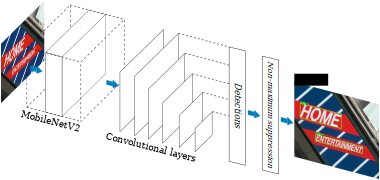
\includegraphics[width=\columnwidth]{ICIP_frankenstein/figs/proposed-method-overview.pdf}
%	\caption{Overview of the proposed method for text localization.}
%	\label{fig:architecture}
%\end{figure}
%\todo[inline]{Move this figure to the "Proposed Method" Section}

% %
% \begin{figure}[!t]
% 	\centering
% 	\includegraphics[height=0.066\textheight]{figs/examples/img_22.jpg}
% %	\includegraphics[height=0.08\textheight]{figs/examples/img_42.jpg}
% %	\includegraphics[height=0.08\textheight]{figs/examples/img_108.jpg}
% 	\includegraphics[height=0.066\textheight]{figs/examples/img_126.jpg}
% 	\includegraphics[height=0.066\textheight]{figs/examples/img_134.jpg}
% 	\includegraphics[height=0.066\textheight]{figs/examples/img_175.jpg}
% 	\caption{Example of challenge scene texts.}
% 	\label{fig:dataset-examples}
% \end{figure}
% %

Among the several approaches for localizing text in images, deep-learning-based techniques are the most promising strategies to reach high detection accuracy. \etal{He}~\cite{He2016TIP}, for example, presented a novel technique for scene text detection by proposing a Convolutional Neural Network (CNN) architecture that focuses on extracting text-related regions and specific characteristics of a text. The authors introduced a deep multi-task learning mechanism to train the Text-CNN efficiently, in which each level of the supervised information (text/non-text label, character label, and character mask) is formulated as a learning task. Besides, the authors proposed a pre-processing method, which extends the widely used Maximally Stable Extremal Regions (MSERs)~\cite{Matas2004IVC} by enhancing the local contrast between text and background regions. %The authors reported significant improvements in terms of recall and precision rates, in comparison with methods designed with traditional machine learning techniques for characterizing and learning high level information~\cite{Minetto2014CVIU}. 
Although the proposed CNN presented a reasonable efficiency in detecting candidate regions, with a processing time of about $0.5$ seconds per image, the pre-processing step requires about $4.1$ seconds per image, which may prevent a real-time detection. 

Another venue that may render outstanding results in terms of effectiveness consists of combining different deep learning architectures to benefit from complementary information to make a better decision. In this vein, \etal{Zhang}~\cite{Zhang2016CVPR} introduced an approach based on two Fully Convolutional Network (FCN) architectures for predicting a salient map of text regions in a holistic manner (named as \textit{Text-Block FCN}), and also for predicting the centroid of each character. The main idea of this approach consists of detecting text line blocks, which are more stable in comparison with character regions. Similarly, \etal{Tang} also proposed an ensemble of three modified VGG-16 networks~\cite{Tang2017TIP}: the first extracts candidate text regions (CTR); % of the scene image;  
the second network refines the coarse CTR detected by the first model, segmenting them into text; and finally, the refined CTR are served to a classification network to filter non-text regions and obtain the final text regions. The CTR extractor network is a modified VGG-16 that, in the training process, receives the edges of the text as supervisory information in the first blocks of convolutional layers and the segmented text regions in the last blocks. %Undoubtedly, 
Both strategies present several issues in terms of computational efficiency that could make their use unfeasible in restrictive computing scenarios.% (e.g., mobile devices).

Towards having a truthfully single-stage text detection, \etal{Liao}~\cite{Liao2018TIP} proposed an end-to-end solution named TextBoxes++, which handles arbitrary orientation of word bounding boxes, whose architecture inherits from the VGG-16 architecture. Similarly to TextBoxes++, \etal{Zhu} proposed a deep learning approach~\cite{Zhu2018TITS} also based on the VGG-16 architecture, but for detecting text-based traffic sign. Both techniques presented outstanding detection rates, but they rely on the use of VGG-16 architecture, which could be considered inadequate for restrictive computing scenarios due to its model size with about $138$ millions of parameters~\cite{Howard2017CoRR}, and floating-point operations per second (FLOPS) that reach about $15.3$ billion~\cite{HeCVPR2016}. In contrast, lighter CNN architectures, such as MobileNet~\cite{Howard2017CoRR}, present a very competitive alternative for this scenario, with a model size of $4.2$ millions of parameters and the FLOPS of $569$ million, for instance.

In light of these remarks, we propose a novel method for text localization considering efficiency and effectiveness trade-offs. Our approach, named MobText, combines two light architectures that were originally proposed for object detection -- MobileNetV2~\cite{Sandler2018CVPR} and SSD~\cite{Liu2016ECCV} -- and adapts them to our problem. The main contributions of this work are: 

\begin{itemize}
    \item (i) the proposal of an effective method for text localization task in scene images, which presented better or competitive results when compared with state-of-the-art methods at a low computational cost in terms of model size and processing time; 
    \item (ii) a comparative study, in the context of text localization, comprising widely used CNN architectures recently proposed for object detection;
    \item (iii) state-of-the-art results on the ICDAR'11 dataset, with F-Measure of $96.09\%$, and competitive results on ICDAR'13 with F-Measure of $73.58\%$; and
    \item (iv) proposal of an evaluation tool to support the assessment of text localization and recognition methods. %\todo[inline]{Provide contribution and adapt introduction to tool description}
\end{itemize}
%; and (iii) a study the most promising deep learning techniques for text recognition task?.

In summary, we addressed the following research questions:
\begin{itemize}
    \item Would a general-purpose object detection network, trained for the text detection task, achieve competitive results, in comparison with state-of-the-art methods?
   % \todo[inline]{Suggestion: Can an object detection network, trained for the text detection task, achieve competitive results, in comparison with state-of-the-art methods?}
    \item Would a mobile-oriented CNN architecture maintain a competitive performance on text detection while being light enough to be executed on devices with restricted computing power and built-in memory capacity?
    %\todo[inline]{Suggestion: Can a mobile-oriented CNN architecture maintain a competitive performance on text detection while being light enough to be executed on devices with restricted computing power and built-in memory capacity?}
    
    \item How to devise a generic evaluation tool to support the assessment of text localization and recognition methods?
\end{itemize}


%\etal{Gupta}~\cite{Gupta2016CVPR} proposed a new method for generating synthetic data for the text spotting problem, by blending synthetic text in natural images in order to have a scene text-like dataset, as illustrated in Figure~\ref{fig:Gupta2016CVPR-pipeline.png}. The authors also proposed a new FCN architecture for text/non-text detection. The SynthText dataset consists of synthetic text-scene images produced by a generation engine that localize the best location in a given image (e.g., contiguous regions) by using segmentation and geometry estimation algorithms and render a synthetic text in the found regions taking into account the local color and texture information to produce realistic scene-text images. The FCN network proposed by the authors based on \etal{Long}~\cite{Long2015CVPR} and \etal{Redmon}~\cite{Redmon2016CVPR} works. According to the authors, the improvements made in the YOLO architecture~\cite{Long2015CVPR} was crucial to achieve good results, in terms of accuracy, at a lower computation cost. The effectiveness of the proposed method was confirmed on ICDAR'11 and ICDAR'13 datasets, whose results were superior to works proposed in~\cite{Wang2012ICPR,Jaderberg2016IJCV,Neumann2012CVPR,Zhang2015CVPR}.

The remaining of this dissertation is organized as follows. Chapter~\ref{chap:related-work} introduces basic concepts related to the text detection problem, along with a brief background of technologies and techniques employed in this dissertation. Chapter~\ref{chap:proposed-method} presents MobText, the proposed method for text detection, besides the datasets, evaluation metrics, and protocols used to validate our approach, in comparison with baselines and their usage in real-world usage scenarios involving the use of mobile devices. This chapter also presents and discusses experimental results. %A description of the experiments made on a mobile, restrictive computing environment is provided in Chapter~\ref{chap:mobile-results}.
Chapter~\ref{chap:tool} describes the developed tool to support the evaluation of text localization and recognition methods.
Chapter~\ref{chap:conclusions} provides our conclusions over the results of our research and points out possible future work. 








\chapter{Concepts and Related Work}%Background and related work
\label{chap:related-work}
This chapter provides an overview of the background and concepts related to this dissertation. Section~\ref{sec:text-localization-recognition}
introduces the main concepts related to text localization and recognition problem. Next, in Section~\ref{sec:deep-learning},  we briefly present a background on deep learning and on its use in the context of restricted computing power scenarios. Finally, examples of efficient and effective methods are discussed.

\section{Text Localization and Recognition}
\label{sec:text-localization-recognition}

Text localization and recognition in images and videos from diverse sources have received substantial attention recently, as diverse ``robust reading'' competitions as ICDAR'11 ~\cite{Karatzas2011ICDAR}, ICDAR'13~\cite{Karatzas2013ICDAR}, and ICDAR'15~\cite{icdar15} emerged as tools to infer the state-of-the-art in methods designed to address this issue.%\todo[inline]{I did not understand the message of this paragraph.}

%\textcolor{red}{Rewrite the paragraph below}
%The main objective can be summarized in determining if there is text in given image, detect it localize it then recognize it. 

The objectives of text localization and recognition are:
\begin{itemize}
    \item To determine if there is a text in a given image;
    \item To find the text location, obtaining the estimated position in the image; and %\todo{tell something about the expected output of this step}
    \item To recognize the text, obtaining the characters or words contained in the text.%\todo{tell something about the expected output of this step}
\end{itemize}

\subsection{Scene Text}
    Given the huge rise in the availability of portable, accessible image recorders as smartphones and cameras, it is possible to notice an equivalent increase in the size of data archives and datasets composed of images. A very common element in digital images is text. Text in digital images can occur in a variable fashion: as artificially generated graphic text, digitally added to an image as a caption; or even in scenarios related to giving some useful context to the image as a timestamp or subtitles; and in scene images, which is naturally found in the image captured by the camera and is part of the scene, like a shop facade or a street sign, for example. 
    
    Graphic, or born-digital images, as is called in ICDAR'11 competition~\cite{Karatzas2011ICDAR}, have some characteristics so that methods can take advantages of them. Commonly, born-digital images have the text horizontally oriented, in the foreground, with high contrast and in a very controlled background. Examples of such images can be found in Figure~\ref{fig:sample_icdar11}. Scene text, as shown in Figure~\ref{fig:sample_icdar13}, is a lot more complex: the text is usually cluttered with the background, with variable texture, color, illumination and orientation. Furthermore, possible deformations derived from a perspective view and occlusions from other objects can also be found.
    %\todo[inline]{Please check if you added a period in every caption in the dissertation}
    \begin{figure}[h!]
    \centering
	\includegraphics[height=0.19\textheight]{dataset_samples/icdar11/img_40.jpg}
	\includegraphics[height=0.19\textheight]{related_work/figs/icdar11_img_33.png}
	\includegraphics[height=0.19\textheight]{related_work/figs/icdar11_img_30.png}

	\vspace{1.5mm}
	
	\includegraphics[height=0.16\textheight]{dataset_samples/icdar11/img_138.jpg}
	\includegraphics[height=0.16\textheight]{dataset_samples/icdar11/img_89.jpg}
	\includegraphics[height=0.16\textheight]{related_work/figs/icdar11_img_64.jpg}

	
	
	\caption{Examples of images with digitally generated text (extracted from the ICDAR'11 dataset~\cite{Karatzas2011ICDAR}).}
	\label{fig:sample_icdar11}
    \end{figure}

    \begin{figure}[h!]
        \centering
    	\includegraphics[height=0.18\textheight]{related_work/figs/icdar13_img_8.jpg}
    	\includegraphics[height=0.18\textheight]{related_work/figs/icdar13_img_5.jpg}
    	\includegraphics[height=0.18\textheight]{related_work/figs/icdar13_img_2.jpg}
    
    	\vspace{1.5mm}
    	
    	\includegraphics[height=0.172\textheight]{related_work/figs/icdar13_img_1.jpg}
    	\includegraphics[height=0.172\textheight]{dataset_samples/icdar13/img_16.jpg}
    	\includegraphics[height=0.172\textheight]{dataset_samples/icdar13/img_83.jpg}
    	
    	\caption{Examples of scene text images (extracted from the ICDAR'13 dataset~\cite{Karatzas2013ICDAR}).}
    	\label{fig:sample_icdar13}
    \end{figure}
    
    \subsection{Text Localization}
    The process of detecting texts present in an image is called text localization. The fundamental goal is to determine which regions of an image contain a textual element, considering the fact that there is no prior information on whether or not the input image contains any text. Found textual elements are often enclosed in bounding-boxes with as minimum background as possible, or the pixels constituting the textual element can be highlighted in a binary mask. In this process, the text in the image is segmented from the background. Figure~\ref{fig:bbox-example} shows examples of outputs of a text localization algorithm\cite{wang2011}.
   % \todo[inline]{Include one or two more example in this Figure. We have space for that.}
    \begin{figure}[h!]
        \centering
    	\includegraphics[height=0.25\textheight]{related_work/figs/example_text_recognition.png}
    	\includegraphics[height=0.25\textheight]{related_work/figs/example_text_recognition2.png}
    	\caption{Examples of bounding boxes delimiting texts in images, with the recognized words above each bounding box~\cite{wang2011}.}
    	\label{fig:bbox-example}
    \end{figure}
    
    \subsection{Text Recognition}
    The objective of the text recognition process is basically the same as those of Optical Character Recognition (OCR) software. Given input digital images or videos, the goal is to identify alphabets, numbers, punctuation marks or special characters, without any human cooperation, and then convert each of the recognized symbols into an appropriate character code. Figure~\ref{fig:bbox-example} shows the recognized characters above the bounding box of the located word. 
    
    \subsection{Text Detection and Recognition Methods}
    A common way of categorizing existing methods for text detection and recognition relies on dividing them into deep-learning and non-deep learning groups. In this work, we are assuming that a deep learning method is a machine learning apparatus so that the feature extraction and the classification modules are both trainable. The remaining methods are therefore classified as non-deep methods, even the ones with a trainable classifier but without trainable feature extraction. 
    
        %\subsubsection{Non-deep methods}
    Several non-deep methods were proposed to solve the problem of text detection and recognition. 
    One category of non-deep text detection methods is based on connected component analysis (CCA).  Being essentially a graph-based algorithm, CCA approaches take a set of connected components of the image, each one of them individually labeled by a heuristic about feature similarity. Pattern recognition methods are often used to analyze the spatial and feature consensus of the connected components and then define text regions. Some approaches~\cite{Lee2010,Kumuda2016,HyungIlKoo2013} rely on statistical models like AdaBoost to learn the CCA models, which significantly improve their robustness.  

    Another category of text detection methods consist of the sliding window classification methods. The principle of these methods is sliding a multiscale window through the image, classifying the regions defined by the sliding window as text and non-text regions. Later, positive regions are then grouped into text regions with morphological operations, conditional random fields, or graph methods~\cite{Lee2011,wang2011,Coates,Ng2011}. This class of methods is simple and adaptive. Nevertheless, they are computationally expensive when a complex classifier is used, and a large number of sliding windows needs to be classified. 
    
    Regarding the text recognition problem, a branch of proposals adopted feature-based methods. Some adopted recognition algorithms based on character segments~\cite{Shi2013,Yao}, others exploited label embedding to match strings and images directly~\cite{Rodriguez-Serrano,Gordo2014,Almazan2014}. Features like Stroke~\cite{Buta2015} and character keypoints~\cite{Phan2013} are also detected for the classification problem. The other great branch of non-deep text recognition solutions opted by decomposing the task into sub-problems, such as text binarization, text line segmentation, character segmentation, single character recognition, and word correction~\cite{Lee2013,QixiangYe,Nomura2005,Chen2004,Karatzas2004}. 
    
   The last class of methods refers to end-to-end solutions. This category of methods integrates text detection and text recognition problems into a single system responsible for both tasks. In some initiatives like~\cite{Felzenszwalb2005}, characters are treated as a special case of object detection, being detected by a Nearest Neighbor algorithm trained with shape descriptors and then grouped into words by using a model that relies on a Pictorial Structure. In another work~\cite{Neumann2013}, the authors proposed a delayed decision approach by keeping multiple segmentation samples from each character until the context of each character is known. The segmentation of detected characters was obtained using extremal regions and decoded recognition results in a dynamic programming algorithm.
        
        %\subsubsection{Deep methods}
        %This section describes some of the deep-learning-based text detection and recognition methods.
        %\textcolor{red}{Provide the meaning of the acronyms}
        %SSTD~\cite{sstd} is a variation of the SSD~\cite{ssd} architecture focused on text detection. This proposal outputs word-level bounding boxes, and can be divided into three parts: the convolutional module, the box prediction module and the text specific module. The convolutional and text specific module are directly inherited from the SSD model. The text specific module can be divided into two modules: a text attention module and a hierarchical inception module. The text attention module is responsible for learning rough spatial text features form the convolutional layers, aiming at reducing false detection, detecting more ambiguous text and improving accuracy. The hierarchical inception module has the task to aggregate multiscale features so that multiscale text can be better detected. 
        %
        %Liao et al.~\cite{textboxes} proposed a fully convolutional network adapted for text detection and recognition, named TextBoxes. The authors approach inherits the VGG16~\cite{vgg} architecture, converting the last two fully-connected layers to convolutional layers by parameter downsampling. Multiple output layers are inserted after the last and some of the intermediate layers, and their outputs are aggregated, afterwards passing in a non-maximal supression process.
        %
        %The TextBoxes approach was later extended as the TextBoxes++~\cite{textboxes++} proposal. The objective was to support the detection of arbitrary oriented bounding boxes. The proposed architecture is also a fully convolutional network. This approach extends the original proposal by predicting an arbitrary quadrilateral as a text bounding box, nos only vertically oriented boxes.
        
        %Another way to perform text detection on images relies on the use of methods originally proposed as object detection techniques. The YOLO V3~\cite{yolov3} (You Only Look Once V3) is a fully convolutional network proposed for object detection that reflects the improvements of the authors over the second version of this method. Being based on the GoogLeNet~\cite{googlenet} model, this proposal predicts bounding boxes and class probabilities directly from full images in one evaluation. The system predicts 4-coordinate bounding boxes using dimension clusters as anchor boxes and predicts an objectness score for each bounding box using logistic regression. 
      
        
        
        
   
   
   
\section{Deep Learning}
\label{sec:deep-learning}
%Aqui introduzo o que é deep learning, dou um overview sobre o assunto (origem, definições de alguns termos mais genéricos, breve histórico)

As the method proposed in this work is a deep learning method, in this section a brief introduction on deep learning is presented, and the most commonly used terms are defined.

Deep learning is a subset of the machine learning methods that allows computer systems to improve itself with experience and data. This class of methods learns how to represent the data with a nested hierarchy of representations, with each representation defined in relation to simpler representations of the data. This procedure exploits many layers of non-linear information for feature extraction and transformation, and pattern analysis and classification~\cite{goodfellow,deepmethods}.

Most deep learning methods are defined in the context of Artificial Neural Networks~(ANN)~\cite{handsonml}. Being inspired by the biological neural network from animal brains~\cite{logicalcalculus}, ANN's are a powerful, scalable, and versatile machine learning architectures, being suitable for tackling complex problems by learning from the complex data fed to it in its training phase. An ANN with a significant number of hidden layers, that is, layers located between the input and output layers, is called Deep Artificial Neural Network~\cite{deepmethods}.  

\subsection{Convolutional Neural Networks}

Being inspired by studies over the visual cortex of the brain, Convolutional Neural Networks (CNN) are an architecture of ANN that are specialized in extracting features and information from images. Proposed back in 1998~\cite{lenet}, the basic building block of CNNs are the convolutional layers. Being based on the mathematical concept of convolution, where a function slides over another, and the integral of the pointwise multiplication is measured, the Convolutional Layer abstracts the same concept: each neuron in a convolutional layer $n$ is connected only to a receptive field in the previous layer $n-1$, not to every pixel in the image. This method allows the network to concentrate on small and localized low-level features in the first layers and then assemble these features at higher-level features on the following layers.



\subsection{Mobile-Oriented Neural Networks}

%Nesta sessão dou um overview sobre redes neurais profundas voltadas para o cenário mobile. Explico os problemas que temos no cenário mobile, como falta de memória, baixo poder de processamento, restrição energética, etc. Exemplifico com alguns trabalhos e como ajudam a contornar os problemas do mobile. Talvez introduzir a arquitetura da MobilenetV2 aqui?

Since the popularization of CNNs with AlexNet~\cite{alexnet}, the general trend has been proposing deeper models with more layers of learnable parameters, with even more complicated operations, aiming to achieve better accuracy on their tasks. However, in mobile or restrictive computing scenarios, these models with a high number of operations and computational footprint were unable to perform their tasks in an acceptable time~\cite{Howard2017CoRR}. 

Some solutions aiming to build smaller and faster CNN architectures were proposed to deal with this problem but maintaining the highly effective detection results observed by state-of-the-art methods. One of the first proposals on the scenario of NN for mobile-oriented applications was the Mobilenet~\cite{Howard2017CoRR}, in which the authors aimed at developing a CNN architecture that was competitive to the state of the art at the time but with a lightweight model, focusing first on reducing processing time but also yielding smaller models. This goal was achieved by using depthwise separable convolutions, an alternative to the classical convolutional layer that fragments it into two: the first layer is called a depthwise convolution, that filters each input channel with a single convolutional filter. The second one is called a pointwise convolution, that applies a $1 \times 1$ convolution with the objective of computing new features by a linear combination of the input channels. This layer is equivalent to a traditional convolutional layer, but with less computational operations.

Sandler et al.~\cite{Sandler2018CVPR} proposed a second version of the Mobilenet architecture, named MobilenetV2. The main contribution of this approach was the Inverted Residual with Linear Bottleneck layer. In this new module, the input is a low-dimensional compressed representation of the data, which is first expanded to a high dimension and filtered with a lightweight depthwise convolution. The results are projected back to a low-dimensional representation with a pointwise convolution. A residual connection is also inserted, connecting each low-resolution representation with the next one. This proposal improves the results of the previous version on various tasks, maintaining its low computational cost nature. The intuition is that the bottlenecks encode the model intermediate inputs and outputs, while the inner layer encapsulates the model ability to transform from lower-level concepts (such as pixels) to higher level descriptors (such as image categories). Finally, as with traditional residual connections, shortcuts enable faster training and better accuracy.

\subsection{Deep Learning for Text Detection and Recognition}
        This section describes some of the deep learning-based text detection and recognition methods.
%        \textcolor{red}{Provide the meaning of the acronyms}
        The Single Shot Text Detector (SSTD)~\cite{He2017ICCV} is a variation of the Single Shot Detector~(SSD)~\cite{Liu2016ECCV} architecture focused on text detection. This proposal outputs word-level bounding boxes, and can be divided into three parts: the convolutional module, the box prediction module and the text specific module. The convolutional and text specific modules are directly inherited from the SSD model. The text specific module can be divided into two modules: a text attention module and a hierarchical inception module. The text attention module, which comprises the convolutional layers, is responsible for learning rough spatial text features. The goal is to reduce false detections and improve the detection of ambiguous text. The hierarchical inception module has the task to aggregate multiscale features so that multiscale text can be better detected. This architecture is illustrated in Figure~\ref{fig:sstd_arch}. %\todo[inline]{Add copyright info to Appendix A}
        
        \begin{figure}[!ht]
            \centering
        	\includegraphics[width=\textwidth]{related_work/figs/SSTD_ARCH.png}
        	\caption{The SSTD architecture, figure extracted from \cite{He2017ICCV}©2017.}
        	\label{fig:sstd_arch}
        \end{figure}
        
        
        
        Liao et al.~\cite{Liao2017AAAI} proposed a fully convolutional network adapted for text detection and recognition, named TextBoxes. The authors approach inherits the VGG16~\cite{vgg} architecture, converting the last two fully-connected layers to convolutional layers by parameter downsampling. Multiple output layers are inserted after the last and some of the intermediate layers, and their outputs are aggregated, afterwards passing in a non-maximal supression process.
        
        The TextBoxes approach was later extended as the TextBoxes++~\cite{Liao2018TIP} proposal. The objective was to support the detection of arbitrary oriented bounding boxes. The proposed architecture is also a fully convolutional network. This approach extends the original proposal by predicting an arbitrary quadrilateral as a text bounding box, not only vertically oriented boxes.
        
        \begin{figure}[!ht]
            \centering
        	\includegraphics[width=\textwidth]{related_work/figs/YOLOV3.png}
        	\caption{Schematic of the YOLO V3 architecture ©2016.}
        	\label{fig:yolov3_arch}
        \end{figure}
        
        Another way to perform text detection on images relies on the use of methods originally proposed as object detection techniques. The YOLO V3 (You Only Look Once V3)~\cite{Redmon2018CoRR}, whose architecture can be seen in Figure~\ref{fig:yolov3_arch}, is a fully convolutional network proposed for object detection that reflects the improvements of the authors over the second version of this method. Being based on the GoogLeNet~\cite{googlenet} model, this proposal predicts bounding boxes and class probabilities directly from full images in one evaluation. The system predicts 4-coordinate bounding boxes using dimension clusters as anchor boxes and predicts an objectness score for each bounding box using logistic regression. 
        
      




%Definir o que é text detection 1.5
%Falar que como os metodos sao baseados em rede, nao irmemos abrodar os nao deep, rederir o artigo x referenciado no survey 
%Text Recognition -> 1  paginas e meia
%Deep learning (O que é rede, camada, neuronio....) 1.5 a 2 paginas
%->Deep learning for lowconstrained computing scenario (varias redes gransed com milhoes de parametros sao  boas em muitas coisas, como resnet, etc, e tem varias redes na leteratura boas para cenario restritivo, e no capitulo seguinte falarei sobre as redes que utilizamos (Olhar mais redes mobile, e soluções shallow now) 4-3
% em related work, falar de propostas da literatura que utilizam redes, e então tecer um caminho até as propostas em rede com cenário restritivo. 5 
%3.1 -> redes para o problema 2
%3.2 -> Iniciativas para contrained scenario 3


\FloatBarrier
\newpage
\chapter{MobText}
\label{chap:proposed-method}


In this chapter, a description of the proposed method is provided. Figure~\ref{fig:architecture} illustrates the overall framework of our approach for text localization, which uses MobileNetV2 as feature extractor and then SSD as multiple text bonding boxes detector. We detail the CNN architectures used, and then explain the learning mechanism used for finding a proper CNN model to the problem. Finally, we present and discuss performed experiments aiming to validate the proposed approach.

\begin{figure}[!ht]
	\centering
	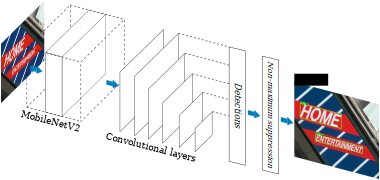
\includegraphics[width=\columnwidth]{ICIP_frankenstein/figs/proposed-method-overview.pdf}
	\caption{Overview of the Proposed Method for Text Localization.}
	\label{fig:architecture}
\end{figure}

\section{Characterization of Text Regions with MobilenetV2}

The MobilenetV2 is a new CNN specifically designed for restricted computing environments that includes two main mechanisms for decreasing the memory footprints and number of operations while keeping the effectiveness of its precursor architecture, the Mobilenet~\cite{Sandler2018CVPR}. Such mechanisms are the linear bottlenecks and the inverted residuals. Besides the depthwise separable convolution operations, which significantly reduce the FLOPS of a neural network, this new version of Mobilenet presents the linear bottleneck mechanism to reduce the number of parameters and keep the accuracy of the network by capturing a low-dimensional subspace (embedded in a manifold formed by a set of activation tensors). The authors claim that non-linearity reduces the capacity of bottleneck features to capture the most representative information. Thus, they decided to use a linear bottleneck, removing the ReLU activation.

The principles that guided the design of the inverted residual layers implemented on MobilenetV2 is that feature maps of the network are able to be encoded in low-dimensional subspaces, and non-linear activation causes some loss of information, notwithstanding their capability to increase representational complexity~\cite{Sandler2018CVPR}.

\begin{figure}[!ht]
	\centering
	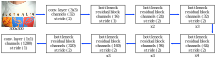
\includegraphics[width=\columnwidth]{ICIP_frankenstein/figs/feature-extraction-v1.pdf}
	\caption{MobilenetV2 architecture used in this work and its parameters. More details on the bottleneck residual block can be found in~\cite{Sandler2018CVPR}.}
	\label{fig:feature-extraction}
\end{figure}

Fig.~\ref{fig:feature-extraction} shows the MobilenetV2 architecture used to characterize text candidate regions. The \textit{bottleneck residual block} implements the optimization mechanisms aforementioned considering the convolutional operations with a kernel of size $3 \times 3$. The first bottleneck block uses an expansion factor of $1$, while the remaining blocks use an expansion factor of $6$, as suggested by \etal{Sandler}~\cite{Sandler2018CVPR}.

\section{Detecting Multiple Instances of Text via SSD}

The localization of text regions in scene images is challenging due to inherent variability of texts, such as size, color, font style, and distortions. 
The text localization should handle multiple scales and bounding boxes with varying aspect ratios. Although several authors consider the image pyramid for performing multi-scale detection, it is quite costly, which may be impractical for a restrictive computing scenario. Thus, we use the Single Shot detector~(SSD) framework~\cite{Liu2016ECCV}, a state-of-the-art method for object detection. The SSD approach includes a multiscale mechanism that allows the identification of text regions in multiple scales on a single inference. Specifically, in the framework, the authors adopt a top-down fusion strategy to build new features with strong semantics while keeping fine details. Text detections are performed based on multiple new constructed features respectively during a single forward pass. All detection results from each layer are refined by means of a non-maximum suppression (NMS) process~\cite{Neubeck2006ICPR}.

\section{Learning}

The main decisions we took in the learning phase of our network are:

\begin{itemize}

\item  {\bf Objective function:}
Similar to \etal{Liu}~\cite{Liu2016ECCV}, we use a multi-task loss function to learn the bounding boxes locations and text/non-text predictions (Equation~\ref{eq:loss}). Specifically, $x_{ij}$ indicates a match ($x_{ij} = 1$) or non-match ($x_{ij} = 0$) between $i$-th default bounding boxes, $j$-th ground-truth bounding boxes, $N$ is the number of matches, $c$ is the ground truth class of the $x_{ij}$ box and the $\alpha$ parameter is used as a multiplier of $\mathcal{L}_{loc}$ to weight the localization loss ($\mathcal{L}_{loc}$) and the confidence loss ($\mathcal{L}_{conf}$). The used loss function can be defined as:
%
\begin{equation}
    L(x,c,l,g) = \frac{1}{N} (\mathcal{L}_{conf}(x,c) + \alpha \mathcal{L}_{loc}(x, l, g))
    \label{eq:loss}
\end{equation}

We adopted the smooth L1 function for $\mathcal{L}_{loc}$ between the predicted box ($l$) and the ground truth box ($g$), and a sigmoid function for $\mathcal{L}_{conf}$. In addition, we set $\alpha=1$ in order to have the localization and confidence components with equal importance.

%\paragraph*{Hard example mining:}
\item {\bf Hard example mining:}
The hard example miner is a mechanism used to prevent imbalances between negative and positive examples during the training phase. On the search for text during the training, we usually have several non-text bounding boxes and few text bounding boxes. To mitigate the training with imbalanced data, we sort the negative bounding boxes according to their confidence, selecting the negative samples with higher confidence value, considering a ratio proportion of 3:1 with the positive samples.

\end{itemize}



%\subsubsection{Linear Bottlenecks}
%
%Beside of depthwise separable convolutions operations, this new version of MobilenetV2 presented the linear bottlenecks in the convolutional blocks aiming reducing the number of parameters of a neural network and capturing the low-dimensional subspace under the supposition that such low-dimensional subspace is embedded in manifold formed by a set of activation tensors. Although the authors did not show a mathematical demonstration that corroborate with this hypothesis, empirical evidences that the use of linear layers is important to prevent non-linearity added from  destroying information. Experiments conducted by the authors shows that non-linear bottlenecks, built with rectified linear units, can decrease the performance significantly in comparison with linear bottlenecks. In other words, the non-linearity can reduce the capacity of bottleneck features in capturing the most representative information.
%
%
%\subsubsection{Inverted residuals bottlenecks} 
%
%For mobile applications and other restrictive computing scenarios, the utilization of computational resources such as memory is crucial since high memory consuming is directly related to battery consumption, besides of provide, in some cases, a negative user experience. To understand how the inverted residual bottlenecks can help in using memory efficiently, we firstly need to understand how the memory-efficient inference works. Basically, a standard implementation builds a directed acyclic compute hyper-graph, in which the nodes represent the tensors and edges represent the operations, and computation (edges) should be scheduled in order to minimize the total number of tensors (nodes).
%


%The SSD-MobilenetV2 model, as described in~\cite{Sandler2018CVPR} was used as a text detector candidate model -- illustrated in Figure~\ref{fig:ssdmobilenet}. The SSDLite is a  mobile-friendly variant of the regular SSD, where the regular convolution layers are replaced by separable convolutions in SSD prediction layers. SSDLite dramatically reduces both parameter count (from 14.8M parameters to 2.1M) and computational cost (1.25B MAdds to 0.25B MAdds) compared to standard SSD. In this model, a Mobilenet V2 is used as a feature extractor for the SSDLite. 
%The MobilenetV2 is a neural network architecture that is designed for mobile and resource-constrained environments, retaining the accuracy of the much bigger and costly models.


\section{Experimental Protocol}
\label{sec:experiments-results}

This section presents the datasets,
metrics, 
and protocols used for evaluating the proposed method.

\subsection{Datasets}
We evaluated the proposed methods in two datasets widely used for evaluating text localization methods, the ICDAR'11 and ICDAR'13. We also used the SynthText dataset to help
training our network due to the small size of the ICDAR's datasets.

\begin{itemize}
    \item {\bf SynthText:} This dataset comprises $858,750$ synthesized text images, which were generated by blending rendered words with natural images~\cite{Gupta2016CVPR}. The synthetic engine proposed by the authors automatically choose the location, in a target image, and transforms a word by using an algorithm that selects contiguous regions based on local color and texture cues. Next, the words were rendered using a randomly selected font,
transformed according to the local surface orientation, and 
finally blended into the scene using the Poisson image editing approach~\cite{Perez2003ToG}.

\item{\bf ICDAR'11:} The ICDAR'11 dataset~\cite{Karatzas2011ICDAR} was introduced in \textit{ICDAR 2011 Robust Reading Competition -- ``Reading Text in Born-Digital Images (Web and Email)''}. 
It is an extension of the dataset used for the text locating competitions of ICDAR 2003~\cite{Lucas2003ICDAR} and ICDAR 2005~\cite{Lucas2005ICDAR}, and contains $551$ images, which were divided into two subsets, 
$410$ images for training and $141$ for test.
The images of this dataset have texts digitally created on them, such as headers, logos, captions, among others. The annotations were built in terms of rectangle word bounding boxes and contains $5,003$ words.

%\paragraph*{ICDAR'13:} 
\item{\bf ICDAR'13:}
This dataset was introduced in \textit{ICDAR 2013 -- ``Focused Scene Text challenge''} and has $462$ images divided into two subsets, training and testing sets, which contains $229$ and $233$ images, respectively~\cite{Karatzas2013ICDAR}. The images in this dataset are born-digital or scene text (captured under a wide variety, such as blur, varying distance to camera, font style and sizes, color, texture, etc). All the text lines are horizontal or near horizontal. The annotations were built in terms of rectangles word bounding boxes and comprise $1,943$ words.

\end{itemize}

\subsection{Evaluation Metrics}

We evaluated the methods in terms of effectiveness and efficiency, according to the metrics described as follow:

\begin{itemize}
\item{\bf  Effectiveness:} We evaluated the effectiveness of the methods in terms of recall, precision, and f-measure. %Here, we consider a correct detection (true positive) if the overlap between the ground-truth annotation and detected bounding box, which is measured by computing the intersection over union, is greater than $50\%$ (similar to standard practice in object recognition~\cite{Everingham2015}). Otherwise, the detected bounding box is considered an incorrect detection (false positive).

\begin{itemize}

      \item \textbf{Intersection over Union (IoU)} is used as protocol to measure the accuracy level between the text detected bounding boxes and the text ground-truth bounding boxes. 
    A detected bounding boxes is considered a correct detection (true positive), if the overlap between the ground-truth annotation and detected bounding box, which is measured by computing the Intersection of Union (Equation~\ref{eq:iou}), is greater than $50\%$. Otherwise, the detected bounding box is considered an incorrect detection (false positive). This protocol was proposed by \etal{Everingham} in the context of the PASCAL VOC challenge~\cite{Everingham2010IJCV} in 2009. Nowadays, it is adopted in ICDAR competitions.
    \begin{equation}
    IoU = \frac{area(B_p \cap B_{gt})}{area(B_p \cup B_{gt})},
    \label{eq:iou}
    \end{equation}
    where $B_p \cap B_{gt}$ and  $B_p \cup B_{gt}$ stand, respectively, for the intersection and the union of the predicted ($B_p$) and ground truth ($B_{gt}$) bounding boxes.
    %
    \item  \textbf{Recall ($R$)} refers to the fraction of text regions correctly detected, given the set of all text regions labeled in the dataset:
    \begin{equation}
        R = \frac{\sum \textrm{true positive}}{\sum (\textrm{true positive + false negative})}
    \end{equation}
    %
    \item  \textbf{Precision ($P$)} refers to the fraction of text regions correctly detected, given all text regions detected by the text detector:
    \begin{equation}
        P = \frac{\sum \textrm{true positive}}{\sum (\textrm{true positive + false positive})}
    \end{equation}
    %
    \item \textbf{F-measure} combines $P$ and $R$, allowing the possibility of having one single effectiveness score to assess the overall quality of a detector. It is defined as:
    \begin{equation}
        \textrm{F-measure} = 2 \times \left( \frac{P \times R}{P + R} \right)
    \end{equation}
    %
  
\end{itemize}

%\todo[inline]{DEFINE THE METRICS!!!!!}

%\paragraph*{Efficiency:} 
\item {\bf Efficiency:} The efficiency aspects considered both the processing time and the disk usage (in MB). We used the Linux {\em time} command to measure the processing time, %since this tool can be applied to all evaluated methods, regardless the programming language.
while the disk usage considered the size of the learned models. %and excluding the disk usage regarding the source code and the possible libraries used by the methods (e.g., Tesseract (tessdata) tool).
All experiments were performed considering a Intel(R) Core(TM) i7-8700 CPU @ 3.20GHz with 12 cores, a Nvidia GTX 1080 TI GPU, and 64GB of RAM.
% \begin{itemize}
%     \item \textit{CPU}: Intel(R) Core(TM) i7-8700 CPU @ 3.20GH;
%     \item \textit{GPU}: Nvidia GTX 1080 ti 11GB and Nvidia GTX Titan X 12GB;
%     \item \textit{Memory RAM}: 62GB;
%     \item \textit{Operating system}: Ubuntu 16.04 LTS (Xenial Xerus).
% \end{itemize}
\end{itemize}

\subsection{Evaluation Protocols}
\label{sec:protocols}

Here, we describe the experimental protocols used for evaluating the proposed method. 

\subsubsection{Comparisons with Baselines}

The experiments were divided into three steps: training, fine-tuning, and test. For the training step, we used three subsets of the SynthText dataset. This dataset comprises of images with synthetic texts added in different backgrounds and we selected samples of the dataset considering $10$ ($9.25\%$), $20$ ($18.48\%$), and $30$ ($27.71\%$) images per background. The resulting subsets were again divided into train and validation, using $70\%$ for training and $30\%$ for validation. Using these collections, we trained a model with random initialization parameters until we found no significant variance in the loss function. For the fine-tuning step, we took the model trained in SynthText and continued this training using ICDAR'11 or ICDAR'13 training subsets, stopping when we found no significant variance in the loss function. Finally, for the test step, we evaluated each fine-tuned model in the test subset of ICDAR'11 or ICDAR'13.

\begin{itemize}
\item {\bf Experimental setup}

We conducted the training of the proposed method considering a single-scale input, and therefore, all input images were resized to $300 \times 300$ pixels. The training phase was performed using a batch size of $24$ and we used the RMSprop optimizer~\cite{Tieleman2012} with a learning rate of $4 \times 10^3$. We also use the regularization L2-norm, with a $\lambda=4 \times 10^5$, to prevent possible over-fitting. We conducted the training until the network converge.



\item{\bf Baselines}


This section provides an overview of the chosen methods for comparison purpose. For a fair comparison, we selected recent approaches specifically designed for a fast detection, including SqueezeDet and YOLOv3. We also use state-of-the-art methods for text localization as baselines.

\begin{itemize}
%\paragraph*{TextBoxes:} 
\item{\bf TextBoxes:} This method consists of a Fully Convolutional Network (FCN) adapted for text detection and recognition~\cite{Liao2017AAAI}. This network uses the VGG-16 network as feature extractor followed by multiple output layers (text-boxes layers), similar to SSD network. At the end, the Non-maximum suppression (NMS) process is applied to the aggregated outputs of all text-box layers. The authors also adopt an extra NMS for multi-scale inputs on the task of text localization.

\item{\bf TextBoxes++:} Liao et al.~\cite{Liao2018TIP} proposed an end-to-end solution able to predict arbitrary orientation word bounding boxes. This architecture is a Fully Convolutional Neural Network (FCN) that detects arbitrary-oriented text. This architecture is inherited from the  popular VGG-16  architecture used for the ImageNet competition. First, the last two FCN layers of VGG16 are converted into convolutional layers (conv6 and conv7). Next, other eight convolution layers divided into four stages (conv8 and conv11) with  different  resolutions  by  max-pooling  are  appended  after conv7. In the following, multiple output layers (text boxes layers) are inserted after the last and intermediate convolutional layers to predict text presence and bounding boxes. Finally, a non-maximum suppression (NMS) process is applied to the aggregated outputs of all text-box layers.

\item {\bf Single-Shot Text Detector (SSTD):} \etal{He}~\cite{He2017ICCV} designed a natural scene text detector that directly outputs word-level bounding boxes without post-processing, except for a simple NMS. The detector can be decomposed into three parts: a convolutional component, a text-specific component, and a box prediction component. The convolutional and box prediction components are inherited from the SSD detector~\cite{Liu2016ECCV} and the authors proposed a text-specific component which consists of a text attention module and a hierarchical inception module.

\item {\bf SqueezeDet:} This network was proposed to detect objects for the autonomous driving problem, which requires a real-time detection~\cite{Wu2017CVPRW}. The SqueezeDet contains a single-stage detection 
% pipeline, which comprises essentially three components: a FCN, a Convolutional layer, and a filtering stage to remove redundant bounding boxes. The FCN is responsible for generating the feature map, while % for the input images. Next, these feature maps are used to feed 
% the convolutional layer %, which 
% is responsible for detecting, localizing, and classifying objects at the same time. The non-maximum suppression (NMS) is also applied to remove the overlapped bounding boxes.
pipeline, which comprises three components: (i) a FCN responsible for generating the feature map for the input images; (ii)  a convolutional layer responsible for detecting, localizing, and classifying objects at the same time; and (iii) the non-maximum suppression (NMS) method, which is applied to remove the overlapped bounding boxes.

\item {\bf YOLOv3:} This is a convolutional network originally proposed for the object detection problem~\cite{Redmon2018CoRR}. Similarly to SSD network, the YOLOv3 predicts bounding boxes and class probabilities, at the same time. The bounding boxes are predicted using dimension clusters as anchor boxes and predicts an objectness score for each bounding box using logistic regression.

\end{itemize}

\end{itemize}

\subsubsection{Experiments on Mobile-Oriented Environment}

This section provides a description of experiments performed on a device with restricted computing capacity. %After a description of the  mobile device technical specifications, the experimental protocol is defined alongside with the data used to evaluate the solution.

To emulate the use of our proposed solution on real-world usage scenarios and to evaluate the performance on a real constrained computing, an Android application was developed and executed. The developed Android application (APP) utilizes TensorFlow~\cite{tensorflow}'s Android API so it can load and execute the same model used for inference in our previous evaluations. 
The chosen portable device for the implementation and execution of our test was a \textit{Xiaomi Redmi Note 5} smartphone, running Android OS version 9 on a \textit{Qualcomm Snapdragon 636} chipset, comprehending a quad-core 1.8Ghz processor alongside a quad-core 1.6Ghz processor and 4 Gb of RAM.

Two sets of experiments where conducted with the goal of assessing the embedded system: 
\begin{enumerate}
    \item Evaluation of the processing time of the proposed approach when running on a mobile device. Experiments considered the detection of images belonging to the ICDAR'11 and ICDAR'13 datasets; and
    \item Evaluation on a real-world mobile-based usage scenarios.
\end{enumerate}

To ensure that the model executed on the mobile device has the same quantitative effectiveness that the one executed on a non-restrictive computing scenario, the same experiments used to evaluate the proposal on the non-restrictive device were executed on the mobile device, conserving datasets and evaluation metric configurations.

The proposed solution was also evaluated in real-world usage scenarios. Given the portability of the embedded APP, the proposed approach was evaluated in detection scenarios involving several images depicting texts in scenes captured using the portable device. To evaluate the efficiency of the proposed method considering a restricted computing environment, we collected $250$ images containing text and non-text elements, captured directly from the built-in camera of the mobile device.

%Mandar para o proximo capitulo
\section{Results}
\label{chap:results}

This section presents and discusses our achieved results, considering the described metrics and experimental protocol. The results of our proposal are compared to state-of-the-art methods. Results regarding the developed mobile application are presented alongside visual examples.

\subsection{Comparisons with Baselines}

This section presents the experimental results of the proposed method (MobText) and a comparison with the state-of-the-art methods for text localization. Table~\ref{tab:comparison-efficacy-deep-learning-methods-icdar11} shows the results for the evaluated methods considering the ICDAR'11 dataset. In this case, the MobText method achieved the best results with Precision, Recall, and F-measure values of $97.40\%$, $94.81\%$, and $96.09\%$, respectively. On the other hand, the SqueezeDet network presented the lowest Precision and F-measure among the evaluated methods ($56.36\%$ and $66.01\%$, respectively). In turn, the TextBoxes achieved the lowest results of Recall ($71.93\%$).
%
\begin{table}[!h]
    \centering
    \caption{Comparison of effectiveness among the evaluated deep learning-based methods for the ICDAR'11 dataset.}
    \label{tab:comparison-efficacy-deep-learning-methods-icdar11}
    \resizebox{0.9\columnwidth}{!}{ 
    \begin{tabular}{lrrr}
        \topline
        \headcol
        \textbf{Methods}       & \textbf{Precision (\%)} &  \textbf{Recall (\%)} &  \textbf{F-measure (\%)} \\ 
        \midline
        MobText        & \highlight{97.40} & \highlight{94.81} & \highlight{96.09} \\ \hline
         SSTD                   & $89.28$           & $78.53$           & $83.56$           \\ \hline
         TextBoxes              & $92.15$           & $71.93$           & $80.80$           \\ \hline
         TextBoxes++            & $95.76$           & $90.51$           & $93.06$           \\ \hline
         YOLOv3                 & $94.27$           & $89.21$           & $91.67$           \\ \hline
         SqueezeDet             & $56.36$           & $79.66$           & $66.01$           \\
       \bottomlinec
    \end{tabular}}
\end{table}

With regard to ICDAR'13 dataset, the SSTD methods presented the highest Recall ($82.19\%$), and F-measure ($86.33\%$), while the YOLOv3 reached the best results in terms of Precision (Table~\ref{tab:comparison-efficacy-deep-learning-methods-icdar13}). Note, however, that the MobText yields very competitive results for this dataset as well, in terms of Precision. 
%In contrast, the SqueezeDet presented the lowest Precision, Recall, and F-measure, with values about $29.41\%$, $62.47\%$, and $39.99\%$, respectively.
%
\begin{table}[!h]
    \centering
    \caption{Comparison of effectiveness among the evaluated deep learning-based methods for the ICDAR'13 dataset.}
    \label{tab:comparison-efficacy-deep-learning-methods-icdar13}
    \resizebox{0.9\columnwidth}{!}{ 
    \begin{tabular}{lrrr}
        \topline
        \headcol
        \textbf{Methods}       & \textbf{Precision (\%)} &  \textbf{Recall (\%)} &  \textbf{F-measure (\%)} \\ 
        \midline
        MobText        & $88.04$           & $63.20$           & $73.58$           \\ \hline
        TextBoxes++            & $90.49$           & $80.82$           & $85.38$           \\ \hline
         SSTD                   & {90.91} & \highlight{82.19} & \highlight{86.33} \\ \hline
         TextBoxes              & $88.84$           & $74.16$           & $80.83$           \\ \hline
         YOLOv3                 & \highlight{92.01}           & $75.71$           & $83.07$           \\ \hline
         SqueezeDet             & $29.41$           & $62.47$           & $39.99$           \\ 
       \bottomlinec
    \end{tabular}}
\end{table}
%
\begin{figure}[!h]
    \centering
    % \includegraphics[height=0.25\textheight]{VISAPP/figs/efficacy-and-efficiency/deep-methods-icdar11-precision.pdf}
    % \includegraphics[height=0.25\textheight]{VISAPP/figs/efficacy-and-efficiency/deep-methods-icdar13-precision.pdf} \\
    % \includegraphics[height=0.25\textheight]{figs/efficacy-and-efficiency/deep-methods-icdar11-recall.pdf}
    % \includegraphics[height=0.25\textheight]{figs/efficacy-and-efficiency/deep-methods-icdar13-recall.pdf} \\
    \includegraphics[width=0.80\textwidth]{ICIP_frankenstein/figs/deep-methods-icdar11-f-measure.png} \\
    \includegraphics[width=0.80\textwidth]{ICIP_frankenstein/figs/deep-methods-icdar13-f-measure.png}
    \caption{Comparison results among the evaluated methods considering aspects of efficacy and efficiency.}
    \label{fig:deep-methods-efficacy-and-efficiency}
\end{figure}

%Now, we will turn our attention for 
In term of 
%evaluating 
the efficiency of the presented methods, 
Fig.~\ref{fig:deep-methods-efficacy-and-efficiency} summarizes the results considering the metrics used to assess the effectiveness of the evaluated methods, in terms of F-measure, along with the metrics for measuring the efficiency of those methods, considering the ICDAR'11 and ICDAR'13 datasets.

Regarding efficiency (processing time and disk usage), the proposed method (MobText) yielded very competitive results, taking only $0.45$ and $0.55$ seconds per image, considering the ICDAR'11 and ICDAR'13, respectively. Comparing MobText with the baseline methods originally proposed for text localization (TextBoxes, TextBoxes++, SSTD), the proposed method presented very competitive results with a processing time of $0.67$ seconds per image and with disk usage of about $37.0$MB. In contrast, the most effective baseline methods, the SSTD and TextBoxes++ networks, presented competitive results in terms of effectiveness and worse results in terms of processing time in comparison with the proposed method. Regarding the disk usage, MobText also presented the best balance between accuracy and model size.   

Now, when compared with the state-of-the-art approaches for object detection, the proposed method also presented competitive results. In this case, the fastest approach for text localization was the SqueezeDet network, which takes about $0.1$ seconds per image, on average. However, when we take into account the trade-off between efficiency and effectiveness, we can safely argue that the proposed method presented a better compromise between these two measures. Figure~\ref{fig:qualitative-results-good-11} provides some cases of success and Figure~\ref{fig:qualitative-results-bad-11} cases of failure of the proposed method for the ICDAR'11 and Figures~\ref{fig:qualitative-results-good-13} and~\ref{fig:qualitative-results-bad-13} for ICDAR'13 datasets. 


\begin{figure}[!h]
	\centering

    \includegraphics[height=0.29\textheight]{VISAPP/figs/qualitative-results/icdar11/69.png}
    \includegraphics[height=0.29\textheight]{VISAPP/figs/qualitative-results/icdar11/46.png}
    
    \vspace{1.5mm}
    
    \includegraphics[height=0.20\textheight]{VISAPP/figs/qualitative-results/icdar11/14.png}
    \includegraphics[height=0.20\textheight]{VISAPP/figs/qualitative-results/icdar11/29.png}
    
    \caption{Examples of success cases of the proposed approach for the ICDAR'11 dataset. Green bounding boxes indicate the regions correctly localized.}
	\label{fig:qualitative-results-good-11}
\end{figure}

%includegraphics[width=0.19\textwidth]{VISAPP/figs/qualitative-results/icdar11/117.png} \\

\begin{figure}[!h]
	\centering

    \includegraphics[height=0.20\textheight]{VISAPP/figs/qualitative-results/icdar11/22m.png}
    \includegraphics[height=0.20\textheight]{VISAPP/figs/qualitative-results/icdar11/53m.png}

    \vspace{1.5mm}

    \includegraphics[height=0.25\textheight]{VISAPP/figs/qualitative-results/icdar11/32m.png}
    \includegraphics[height=0.25\textheight]{VISAPP/figs/qualitative-results/icdar11/10m.png}

\caption{Examples of failure cases of the proposed approach for the ICDAR'11 dataset. Green bounding boxes indicate the regions correctly localized, while red bounding boxes show candidate regions not detected by our method.}
	\label{fig:qualitative-results-bad-11}
\end{figure}

\begin{figure}[!h]
	\centering

    \includegraphics[height=0.20\textheight]{VISAPP/figs/qualitative-results/icdar13/19.png}
    \includegraphics[height=0.20\textheight]{VISAPP/figs/qualitative-results/icdar13/83.png}
    
    \vspace{1.5mm}
    
    \includegraphics[height=0.20\textheight]{VISAPP/figs/qualitative-results/icdar13/129.png}
    \includegraphics[height=0.20\textheight]{VISAPP/figs/qualitative-results/icdar13/140.png}
	\caption{Examples of success cases of the proposed approach for the ICDAR'13 dataset. Green bounding boxes indicate the regions correctly localized.}
	\label{fig:qualitative-results-good-13}
\end{figure}
\begin{figure}[!h]
	\centering
    
    \includegraphics[height=0.20\textheight]{VISAPP/figs/qualitative-results/icdar13/1m_crop.png}
    \includegraphics[height=0.20\textheight]{VISAPP/figs/qualitative-results/icdar13/18m.png}

    \vspace{1.5mm}

    \includegraphics[height=0.20\textheight]{VISAPP/figs/qualitative-results/icdar13/41m.png}
    \includegraphics[height=0.20\textheight]{VISAPP/figs/qualitative-results/icdar13/48m.png}
%   \includegraphics[height=0.20\textheight]{VISAPP/figs/qualitative-results/icdar13/49m.png}

	\caption{Examples of failure cases of the proposed approach for the ICDAR'13 dataset. Green bounding boxes indicate the regions correctly localized, while red bounding boxes show candidate regions were not detected by our method.}
	\label{fig:qualitative-results-bad-13}
\end{figure}

The proposed method is able to detect multi-oriented texts and even texts with textured backgrounds. However, as we could observe, the proposed approach presented some difficulties in localizing scene text in the ICDAR'13 dataset. In comparison with results achieved for the ICDAR'11, the precision and recall rates decreased $9.36$ and $31.61$ percentage points, respectively, which suggest that our network did not localized several candidate regions containing texts.

\begin{figure}[!h]
    \centering
    \includegraphics[width=0.75\textwidth]{VISAPP/figs/boxplot_error_icdar13.pdf}
    \caption{Comparison among distributions of relative areas of bounding boxes from Ground-Truth (GT), False Negatives (FN) cases, and False Positive (FP) cases. We omitted the points considered outliers for a better visualization.}
    \label{fig:boxplot}
\end{figure}

To understand the reasons that led the proposed method to have this difficult in localizing text for the ICDAR'13 datasets, we performed an analysis of failure cases taking into account the relative area of missed bounding boxes. Figure~\ref{fig:boxplot} presents a box-plot graph that shows the distribution of the relative area of bounding boxes (i.e., ratio of bounding box area to image area) for the ground-truth, false positive cases, and false negative cases.

\begin{figure}[!h]
    \centering
    %\includegraphics[width=\columnwidth]{version-2/figs/small_box.jpg}
    \includegraphics[width=0.99\textwidth]{VISAPP/figs/hires_samples.png}
    \caption{Two high resolution examples of ICDAR'13 dataset with both medium-sized text (detected by our method) and small-sized (not detected).}
    \label{fig:small_example}
\end{figure}

As we can observe, the missed bounding boxes (false negative cases) have a small relative area. More precisely, $75\%$ of false negative cases (third quartile of FN box-plot) have a relative area up to $0.01$ and correspond to $50\%$ of the bounding box present in the ground-truth (median of GT box-plot). This results suggest to us that high resolution images with relatively small text (see Fig.~\ref{fig:small_example}) are specially challenging to our method. To overcome this limitation, future investigations can be conducted to devise an architecture to better localize bounding boxes with multiple scales such as Feature Pyramid Networks (FPNs), as proposed by \citep{Lin2017CVPR}.

\subsection{Results on Mobile-Oriented Environment}

In terms of precision, recall, and F-Measure on ICDAR'11 and ICDAR'13 datasets, the proposal achieved the same results as on the non-restrictive scenario. Table~\ref{tab:times_dataset} shows the efficiency of the network in terms of inference time on both datasets. 

\begin{table}[!h]
    \centering
    \caption{Processing time of the embedded application on ICDAR datasets.}
    \label{tab:times_dataset}
    \begin{tabular}{lrrr}
        \toprule
        \ml{2}{*}{\textbf{Dataset}} & \mcol{3}{c}{\textbf{Processing Time (ms)}}  \\ 
                                    & \textbf{Min.} &  \textbf{Max.} &  \textbf{Average} \\ 
        \midrule
        ICDAR'11                    & $420$         & $524$          & $464$           \\ \hline
        ICDAR'13                    & $449$         & $602$          & $523$           \\
        
       \bottomrule
    \end{tabular}
\end{table}

As we are unable to evaluate the method in a quantitative manner regarding effectiveness on the images captured in the wild, the proposed solution was only evaluated in terms of efficiency, in processing time. A qualitative analysis was performed by taking into account the visual results of the detection on the images. 

 The average time of inference in $250$ images was $425$ms, with a minimum inference time of $343$ms and a maximum of $584$ms.


%%%%%%%%%%%%%%%%%
\begin{figure}[h!]
\centering
\includegraphics[width=0.49\textwidth]{Mobile/images/app27.jpg}
\includegraphics[width=0.49\textwidth]{Mobile/images/app28.jpg}

\caption{Example of scene text images captured with a perspective.}
\label{fig:ic-perspective}
\end{figure}
%%%%%%%%%%%%%%%%%%
Figure~\ref{fig:ic-perspective} shows the effect of the capturing angle of the texts in scene text images. As the system was only trained with horizontal aligned text, this kind of perspective lowers the system effectiveness.


\begin{figure}[h!]
\centering
\includegraphics[width=0.49\textwidth]{Mobile/images/app24.jpg}
\includegraphics[width=0.49\textwidth]{Mobile/images/app25.jpg}

\vspace{1.5mm}

\includegraphics[width=0.49\textwidth]{Mobile/images/app23.jpg}
\includegraphics[width=0.49\textwidth]{Mobile/images/app26.jpg}


\caption{Example of scene text images captured with different zoom levels.}
\label{fig:ic-zoom}
\end{figure}
%%%%%%%%%%%%%%%%%
In Figure~\ref{fig:ic-zoom}, the effects of the size of the text on scene text images is shown. Images with smaller text (top left) are more difficult to detect, while image with medium to big text are easier and have better results, as shown in Figure~\ref{fig:sample_good}. 



\begin{figure}[h!]
\centering
\includegraphics[width=0.49\textwidth]{Mobile/images/app03.jpg}
\includegraphics[width=0.49\textwidth]{Mobile/images/app09.jpg}

\vspace{1.5mm}

\includegraphics[width=0.49\textwidth]{Mobile/images/app07.jpg}
\includegraphics[width=0.49\textwidth]{Mobile/images/app11.jpg}


\caption{Example of scene text images with good results on our application.}
\label{fig:sample_good}
\end{figure}
%%%%%%%%%%%%%%%%%

Even though the system was not trained with handwritten text, the results of text detection on handwritten text, such as in Figure~\ref{fig:handwritten}, are very promising. Good detection results were obtained on handwritten text on a complex background (top left) and even on multilingual text (bottom left). 
\begin{figure}[h!]
\centering
\includegraphics[width=0.49\textwidth]{Mobile/images/app22.jpg}
\includegraphics[width=0.49\textwidth]{Mobile/images/app31.jpg}

\vspace{1.5mm}

\includegraphics[width=0.49\textwidth]{Mobile/images/app17.jpg}
\includegraphics[width=0.49\textwidth]{Mobile/images/app18.jpg}


\caption{Example of handwritten text, with complex backgrounds and multilingual text.}
\label{fig:handwritten}
\end{figure}

%\begin{figure}[!t]
%	\centering
%	\hspace{0.1mm}
%	\includegraphics[height=0.27\columnwidth]{ICIP_frankenstein/figs/qualitative-results/icdar11-success-69.png}
%	\includegraphics[height=0.27\columnwidth]{ICIP_frankenstein/figs/qualitative-results/icdar13-success-5.png}
%    \\ \vspace{0.5mm}
%	\includegraphics[height=0.27\columnwidth]{ICIP_frankenstein/figs/qualitative-results/icdar11-failure-10.png}
%	\includegraphics[height=0.27\columnwidth]{ICIP_frankenstein/figs/qualitative-results/icdar13-failure-185.png}
%	\caption{Examples of success (first line) and failure (second line) cases of the proposed approach for the ICDAR'11 (first column) and ICDAR'13 (second column) datasets.}
%	\label{fig:qualitative-results}
%\end{figure}



% Regarding the efficiency, in terms of processing time, the proposed method presented a very competitive results, taking only $0.09$ seconds per image, on average. This obtained processing time meets the results presented by the authors, which reported a computing speed about $0.02$ seconds per frame, considering an input image of $1,242 \times 375$ pixels.  For the disk usage performance, the lighter deep learning-based model was produced by SqueezeDet, with a size of $23.10$MB. On the other hand, the heaviest deep learning-based model was produced by SSTD network, with a size of $248.20$MB.
%
%\todo[inline]{Include the values for YOLOv3 in the table below}
%
% \begin{table}[!t]
%     \centering
%     \caption{Processing time per image, in seconds, for the evaluated deep learning-based methods.}
%     \label{tab:comparison-efficiency-time-proc-deep-methods-icdar11-icdar13}
%     \resizebox{\columnwidth}{!}{ 
%     \begin{tabular}{lrrr}
%         \topline
%         \headcol
%         \headcol \textbf{Methods} & \textbf{ICDAR'11} & \textbf{ICDAR'13} & \textbf{Average} \\
%         \midline
%         SSTD                      & $0.45$               & $0.55$               & $0.50$              \\ \hline
%         TextBoxes                 & $0.45$               & $0.53$               & $0.49$              \\ \hline
%         TextBoxes++               & $1.70$               & $1.87$               & $1.79$              \\ \hline
%         MobText           & $5.62$               & $4.32$               & $4.97$              \\ \hline
%         % YOLOv3                    & $6.84$               & $7.42$               & $7.13$              \\ \hline
%         % SqueezeDet                & $0.08$               & $0.09$               & $0.09$              \\
%       \bottomlinec
%     \end{tabular}}
% \end{table}
% %		
% \begin{table}[!t]
%     \centering
%     \caption{Comparison of efficiency, in terms of disk usage, among the evaluated deep learning-based methods.}
%     \label{tab:comparison-efficiency-disk-usage-deep-methods}
%     \begin{tabular}{lr}
%         \topline
%         \headcol \textbf{Methods} & \textbf{Disk usage (MB)}    \\
%         \midline
%         SSTD                      & $248.20$                    \\ \hline
%         TextBoxes                 & $95.10$                     \\ \hline
%         TextBoxes++               & $139.10$                    \\ \hline
%         MobText           & $37.00$                     \\ \hline
%         % YOLOv3                    & $246.30$                    \\ \hline
%         % SqueezeDet                & $23.10$                     \\
%       \bottomlinec
%     \end{tabular}
% \end{table}
 %chap4: validatiion  4.1 experimental protocol 4.2Results and discussion
\chapter{Evaluation Tool}
\label{chap:tool}

In this chapter, we present a tool that encompasses traditional and recent methods proposed for text localization and recognition problems, considering both non-deep and deep-learning-based approaches. We also present architectural and functional overviews of the tool, as well as describe deployment procedures and possible usage scenarios.

The developed docker-based tool is composed of three modules: \textit{text spotting}, \textit{post-processing}, and \textit{text recognition} modules. Fig.~\ref{fig:prototype-overview-simple} provides a conceptual overview of the prototype and its components. The text spotting applications refer to methods used for detecting candidate regions in a scene, while the post-processing methods are used to refine detection results. The module dedicated to text recognition applications includes a set of methods that focus on the recognition of texts, given a detected text region image. We provide a command-line interface that enables the creation of all docker images utilized in this prototype, and supports the execution of combinations of the components provided in the three modules. In such a way, text spotting and end-to-end recognition applications may be created and executed independently, depending on the users' needs.

\begin{figure}[h!]
  \centering
  \includegraphics[width=0.6\textwidth]{E4/version-2/figs/prototype-overview-simple.pdf}
  \caption{Overview of the main components of the prototype. The text spotting applications refer to methods used for detecting candidate regions in a scene, while the post-processing applications are used to refine detection results. The text recognition applications provide the components responsible for recognizing texts found within detected regions.}
  \label{fig:prototype-overview-simple}
\end{figure}

\section{Architectural Overview}

The text recognition applications provide the components responsible for recognizing the text found within detected regions. The text localization module includes container applications that encapsulate the text localization methods used for comparison. The post-processing module comprises two containers: the post-processing method developed by the Samsung Research (SRBR) team, and an improved version. Similarly, the text recognition module provides three containers that encapsulate the three recognition methods: Tesseract, Long Short-Term Memory (LSTM), and Convolutional Recurrence Neural Network (CRNN) recognition methods. Table~\ref{tab:methods-available} summarizes the text detection and recognition methods handled in the tool.


\begin{table}[H]
  \centering
  \caption{Method for text detection and recognition available in the evaluation tool. For more detail refer to \cite{joselito}}
  \label{tab:methods-available}
  \begin{tabular}{lp{4.3cm}|p{4.3cm}}
    \hline
    \topline
    \headcol
    \textbf{Type}  & \textbf{Methods for Text Detection}    & \textbf{Methods for Text Recognition} \\ \midline
    & - SnooperText               	& - Tesseract v.3             \\
    & - Canny Text Detection          & \\
    & - MSER-SWT Text Detection         &  - Tesseract with Post-processing \\
   % & - Multi-Lingual Text Detection      & - Tesseract with Improved Post-processing \\
    & - FASText                 &                    \\
    
    \ml{-6}{*}{Non-Deep Methods}
    & - Scene Text Recognition &                    \\ \hline \hline
    & - SSTD                    & - LSTM (Tesseract v.4)         \\
    & - TextBoxes                 & - CRNN                 \\
    & - TextBoxes++                &                    \\
    & - SSD-MobilenetV2              &                    \\
    & - YOLOv3                   &                    \\
    
    \ml{-6}{*}{Deep Learning-Based 
      Methods}    & - SqueezeDet                 &                    \\
    \bottomlinec
  \end{tabular}
\end{table}

%\todo[inline]{Provide a description of said methods. Ask @Allan what is MSER-SWT and "Scene text recognition"
%R.: These are two non-deep methods for text localization that we exploit in the Deliverable E3. @Decker: You can found a description for these methods in the documents that I sent to you yesterday.}

\section{Implemented non-deep methods}

%\todo[inline]{Trocar tudo por uma versao da tabela do E1 e citar o joselito}
This section describes the non-deep methods implemented on the comparative tool. The deep-learning-based methods where already described in Section~\ref{sec:protocols}. Table~\ref{tab:non-deep-methods} presents the non-deep-learning methods considered in the tool. As we can observe, used methods include both region- and component-based approaches. Most of the methods rely on the use of classification systems that exploit shape and/or texture features in the identification of text regions.

\newpage

%\begin{landscape} % for rotate the page
  
  \begin{footnotesize}
    \begin{longtable}{p{.20\textwidth}|p{.20\textwidth}|p{.20\textwidth}|p{.20\textwidth}}
      \caption{Overview upon non-deep-based methods implemented on the comparative tool. For more details please refer to \cite{joselito}.}
      \label{tab:non-deep-methods}
      \endfirsthead
      \endhead
      \topline
      \headcol
       \bf Reference      
      & \bf Type 
      & \bf Features        
      & \bf Classifiers \\
       \midline
  
  
  Snooper text~\cite{Minetto2014CVIU}   
      & Region-based
      & Character filtering: Fourier descriptor, Pseudo-Zernike moments, and Polar descriptor. \newline
      Classification of text and non-text regions: T-HOG~\cite{Minetto2013PR}  
      & Character filtering: ensemble of SVM classifiers. \newline
      Classification of text and non-text regions: SVM \\\hline
  
    FASText~\cite{Buta2015} 
 
      & Component-based
      & Stroke-specific keypoint features
      & Adaboost classifier\\ \hline


  Canny~\cite{Cho2016CVPR} 

      & Component-based
      & Mean local binary pattern (MLBP) 
      & Two-round text classification with AdaBoost and multiple cascades
       \\ \hline
  
  MSER-SWT~\cite{Epshtein2010CVPR} 

      & Region-based and \newline Component-based
      & Stroke Width Transform 
      & Rules and thresholds based on the variance of the stroke
       \\ \hline
       
  Scene Text Recognition~\cite{Neumann2012CVPR} 

      & Component-based
      & Incrementally Computable Descriptors 
      & AdaBoost and SVM
       \\ \hline
      \bottomlinec

      %  \end{tabular}
      %\end{table}
    % \label{tab:non-deep}
    \end{longtable}
  \end{footnotesize}

\subsection{Recognition methods}
Three main recognition methods were implemented in the comparative tool: Tesseract, an LSTM-based approach and a CRNN-based approach. Tesseract~\cite{Smith2007ICDAR} is an open-source OCR engine proposed to recognize words from gray or RGB images, which can be understood as a five-stage pipeline. CRNN combines two types of neural networks, DCNN and RNN, to build an end-to-end system for sequence recognition, and T-LSTM is a Long Short-Term Memory (LSTM) network designed to recognize text lines. The LSTM is a special kind of Recurrent Neural Network (RNN) with the ability of learning long-term dependencies. The use of text recognition approaches is out of the scope of this dissertation. Readers may refer to~\cite{joselito} for a detailed description of such methods. 

\section{Implementation Overview}

The prototype developed in this chapter contains several applications with different software dependencies, including libraries, programming tools, and the base operating system. The integration of all these pieces of software into a single prototype is very challenging and we opted to package all applications that compose the prototype using the Docker\footnote{\url{https://www.docker.com/} (As of Jan 2020).} technology. Docker is an open source platform for operating-system-level virtualization. Docker provides a standardized unit software for packaging the source code and all its dependencies, including system tools, system libraries, and settings.

In this tool, we implement \textit{Dockerfiles}\footnote{Docker building configuration files.} that automatically package the source code, install its dependencies, install and compile source codes, and finally builds a docker image able to run the application as a command line, in a proper software platform. Figure~\ref{fig:overview-prototype} illustrates an overview of the architecture of the prototype. We built two base docker images, which contain some common libraries required for running non-deep- and deep-learning-based methods. These base docker images are used to build the docker images for the applications.
%\todo[inline]{padronizar ao longo da dissertação o uso de Figure and Fig.}
%
\begin{figure}[h!]
  \centering
  \includegraphics[width=0.98\textwidth]{E4/version-2/figs/prototype-overview.pdf}
  \caption{Architectural overview of the prototype.}
  \label{fig:overview-prototype}
\end{figure}

An overview regarding the use of the proposed tool in the context of the evaluation of text detection methods can be found in Appendix~\ref{app:code}.

%\todo[inline]{Incluir no apendice um exemplo de uso do megazord}


%SnooperText is a text detection approach introduced in~\cite{snooper}. This detector is composed of four main steps: image segmentation, character filtering, character grouping, and text region filtering. Initially, it locates candidate characters on images by means of a segmentation and a character/non-character binary classification system. The segmentation approach takes advantages of morphological operations for local contrast enhancement and thresholding. The classification system relies on shape descriptors (e.g., Fourier descriptors, Pseudo-Zernike moments, and Polar descriptor) and an ensemble of SVM classifiers. The candidate characters, represented by their bounding boxes, are then grouped according to geometric criteria. The resulting groups, i.e., candidate text regions, are validated by means of another texture-based classification system, which exploits a multi-cell histogram of oriented gradients (named T-HOG)~\cite{thog}, and another SVM~\cite{svm} classifier. All those steps are performed in multi-scale manner to address issues related to different character sizes and to avoid non-relevant texture details found within character regions.

%\subsection{Canny Text Detection}
%In this work, the authors present a novel scene text detection algorithm, Canny text detector~\cite{cannyTD}, which takes advantage of similarity between image. The proposed method can be summarized in five steps. In the first step, character candidates are extracted using extremal regions (ERs) method. YCrCb space color was used separately to extract ERs, as well their inverted channels. In the second step, a non-maximum suppression process is applied to reduce all repeating components produced by ER. In the third step, a double threshold classification is performed to classify surviving character candidates into three classes: strong text, weak text and non-text. Each character candidate is evaluated using an Adaboost classifier with multiple cascades. Two blocks of cascade classifiers are used, each with a threshold value of 99.0\% and 90.0\%. Mean Local binary pattern (MLBP) is used as the descriptor, which is robust to illumination and rotation variations. In the double threshold classification, all candidates go through the first cascade block and are classified as strong text or non-strong text. Non-strong text candidates go through the second cascade block, which in turn classifies them as weak or non-text. In the fourth step, a text-tracking-based on hysteresis is applied, strong text are included in the final result because they are classified with high confidence. Weak text can be either classified as true text or not-text, so they are included as high confidence if they have similar properties to strong text candidates. In the fifth step, a text grouping process is applied, two candidates are compared based on spatial location, size, color, and aspect ratio using the same threshold values (99.0\% and 90.0\%). If they satisfy the properties, then they are grouped into a same word.

%\subsection{FASText}

%Busta et al.~\cite{fastext} introduced FASText. FASText is a stroke detector based on an efficient pixel intensity comparison to surrounding pixels. FASText is based on four main steps. In the first step, to detect stroke-specific keypoints efficiently, two keypoints classes were introduced: the stroke Ending Keypoint (SEK) fires on a stroke ending, whilst the Stroke Bend Keypoint (SBK) fires on a curved segment of a stroke. Four parameters are used to detect keypoints: circle size, margin, scaling factor, and the maximum number of keypoints. In a second step, a threshold value is found directly from FASText keypoint to segment individual characters from the background. In the third step, to reduce false detection, an efficient classification component is employed. Inspired by the MSER segmentation classifier~\cite{Neumann2015ICDAR}, an AdaBoost is used as a classifier. Compactness, convex hull are ratio, holes area ratio and the character Stroke Area (CSA) are used as features to classify FASText regions as a character or background clutter. CSA feature is based on the observation that the area of an ideal stroke is the product of the stroke width and the length of the stroke.
%In the fourth step, an unordered set of FASText regions classified as text fragment (characters) are clustered together to form lines of text. A standard (approximate) nearest-neighbor algorithm is used for this process.

%\subsection{Scene Text Detection}
%Yi et al.~\cite{Yi2014TIP} address the problem of performing scene text detection and recognition in mobile devices. Character detection is based on the combination of bags of visual words and Gaussian mixture models computed based on HOG features extracted from points defined by four different detectors. Later, stroke configuration maps, defined in terms of character boundary and skeleton, are used to model the character structure for different classes. Target applications refer to text understanding and retrieval.

%\subsection{Multi-lingual}
%33333This proposal~\cite{multilingual} presents a technique for multi-lingual video text recognition which involves script identification in the first stage followed by word and character recognition and finally the results are refined using a post-processing technique. Considering the inherent problems in videos, a Spatial Pyramid Matching (SPM) based technique, using patch-based SIFT descriptors and SVM classifier, is employed for script identification. In the next stage, a Hidden Markov Model (HMM) based approach is used for word and character recognition, which utilizes the context information. Finally, a lexicon-based post-processing technique is applied to verify and refine the word recognition results.

%\subsection{Tesseract}

%Tesseract~\cite{Smith2007ICDAR} is an open-source OCR engine proposed to recognize words from gray or RGB images, which can be understood as a five-stage pipeline. Firstly, the input image (text region) is converted to a binary image using an adaptive threshold. This image is segmented via a connected component analysis method for further inspection of the nesting of outline and also to deal with write-on-black text regions. At this point, the Tesseract provides a set of blobs with nested outlines gather together in order to have an organization of text line regions. The next stage of the method consists of finding text lines by filtering out regions with a height smaller than a threshold $\delta$, which is defined as the fraction of the median height of the text size in that region. Later, the Least Median of Square method~\cite{Rousseeuw1987Wiley} is applied in order to find the baselines and a fixed and non-fixed pitch detection is applied to split words into characters. Finally, a two-step classification process is used to recognize characters, considering a set of topological features~\cite{Shillman1974MIT,Blesser1976PR}, such as y-position relative to baseline, contour length, second x-moment, and second y-moment.
\chapter{Conclusions}


\label{chap:conclusions}

 \nobibliography*

How to perform efficient and effective text detection in scene images in restrictive computing environments? 
To address this research problem, we presented a new method based on the combination of two light architectures, MobileNetV2 and Single Shot Detector~(SSD), which yielded better or comparable effectiveness performance when compared with state-of-the-art baselines despite having a low processing time and small model size, being suitable for a restrictive computing environment.

This work resulted on a published conference paper~\cite{decker}:
\begin{itemize}
    \item \textbf{\bibentry{decker}}.
\end{itemize}

Also, this work contributed to other publications~\cite{joselito-paper,manuel,jhonny}. Appendix~\ref{appendix:A} comprehends a copyright disclaimer for partial use of indexed articles on dissertationsor thesis.


As contributions and answers to our research questions, we have that: 

\begin{itemize}
    \item \textbf{Would an object detection network, trained for the text detection task, achieve competitive results, in comparison with state-of-the-art methods?}
    
    \textbf{Yes}. Compared with other object detection solutions, our method is the most promising one in all evaluation criteria, yielding state-of-the-art on ICDAR'11 dataset and competitive results in ICDAR'13, alongside very satisfactory results on images obtained from the wild. Our findings disagree with the discussion provided in~\cite{Ye2015PAMI}, as we demonstrated that adapting object detector networks for text detection is a promising research venue, besides the system still being sensitive to visual abnormalities such as reflections and deformations.
    
    \item \textbf{Would a mobile-oriented CNN architecture maintain a competitive performance on text detection while being light enough to be executed on devices with restricted computing power and built-in memory capacity?}
    
    \textbf{Yes.} Our method, when executed on a real application on a mobile, computational restrictive device, maintained the performance and had very promising processing time, showing itself suitable for being applied on a embedded system. 
    
    \item \textbf{How to devise a generic evaluation tool to support the assessment of text localization and recognition methods?}
    
     Two types of approaches were considered in the implementation of text detection and recognition approaches: methods that do not rely on deep learning strategies; and methods that take advantage of deep learning-based architectures. The prototype also includes post-processing components, which may be used to improve text detection results.
    
    
\end{itemize}

There is still a lot of work to be done with the scenario of text detection and recognition in devices with restricted computing power that can be a future work after our proposal, such as:

\begin{itemize}
    \item Improve the system to detect multi-oriented text, extending the capabilities of the proposal to multi-oriented text dataset such as ICDAR'15.
    
    \item Improve the architecture of the feature extractor network, aiming for a smaller processing time, consequently a smaller energy impact, and/or the extraction of better features, allowing to detect text on images with abnormalities.
    
    \item Extend the proposed approach for the detection of multi-language text. The goal is to efficiently recognize characters and sentences in languages different from the Latin-derived, such as Chinese, Japanese, Korean, Hindi and Arabic. 
    
    \item Create mobile-based applications that can benefit from the proposed lightweight architecture.
    
    \item Extend the evaluation tool to encapsulate different evaluation protocols, including, among others, datasets, and performance evaluation metrics. 
    
    \item Extend the evaluation tool to simulate scenarios commonly found when handling restrictive computing devices. This infrastructure may contribute, for example, to speed up the development of new text localization and recognition methods customized for specific constrained hardware configurations.
    
    \item Extend the evaluation tool to include a graphical user interface, which would support the selection of text detection and recognition methods.
    
    \item Extend the evaluation tool to support the creation of new applications based on implemented methods. One starting point would be the creation of an application that exploits contextual information provided by text recognition methods.
    
    \item Extend the evaluation tool to support fusion strategies of the different methods for text spotting and recognition.
    
\end{itemize}



% As referências:
\bibliographystyle{ieeetr}
%\bibliography{ic-tese-v3,bib/IEEEabrv,bib/others-abbrev,bib/maestro-samsung,bib/maestro-samsung-idar-ijdar}
\bibliography{new_bib}


% Os anexos, se houver, vêm depois das referências:
\appendix
\chapter{Copyright}
\label{appendix:A}
\begin{figure}[h!]
    \centering
    \includegraphics[width=0.99\textwidth]{related_work/figs/copyright.png}
    \caption{IEEE Copyright disclaimer for partial use of indexed articles on dissertations or thesis.}
    \label{fig:copyright}
\end{figure}
\chapter{Usage Example of the Evaluation Tool}
\label{app:code}
We provide shell scripts to run a text spotting application by choosing the method to be used to detect the candidate regions and also to run all text spotting methods available in the comparative tool. The option to run post-processing methods on top of text spotting method's output is also available.  

To run all text spotting methods available, the following command can be used:

\begin{lstlisting}[style=fancyterminal]
 $ ./1-main-text-spotting-methods.sh \
        --dataset_path /path/to/datasets \
        --working_path /path/to/working/directory/ \
        --dataset_id icdarXX \
        --text_spotting_method_id all-methods
\end{lstlisting}

To see all options available, the following command can be used:
\begin{lstlisting}[style=fancyterminal]
 $ ./1-main-text-spotting-methods.sh --help
 Usage: ./1-main-text-spotting-methods.sh [options]
 
 options:
 -h, --help                show brief help
 --dataset_path            path to dataset directory
 --working_path            path to output directory
 --dataset_id              dataset identifier (choose from icdar11, icdar13, icdar15)
 --text_spotting_method_id text spotting method identifier (choose from options below)
       options:
           all-methods (default)
           deliverable-e2-canny
           deliverable-e2-snoopertext
           deliverable-e4-canny
           deliverable-e4-snoopertext
           deliverable-e4-mserswt
           deliverable-e4-multiligual
           deliverable-e4-scenetext
           deliverable-e4-ssd-mobilenetv2
           deliverable-e4-sstd
           deliverable-e4-squeezedet
           deliverable-e4-yolov3
\end{lstlisting}

To run the post-processing methods available on top of all text spotting methods, the following command can be used:

\begin{lstlisting}[style=fancyterminal]
 $ ./2-main-postprocessing.sh  
        --dataset_path /path/to/datasets \
        --working_path /path/to/working/directory/ \
        --dataset_id icdarXX \
        --text_spotting_method_id all-methods \
        --postprocessing_method_id all-methods
\end{lstlisting}

To see all options available, the following command can be used:
\begin{lstlisting}[style=fancyterminal]
 $ ./2-main-postprocessing.sh --help
 Usage: ./2-main-postprocessing.sh [options]
 
 options:
 -h, --help                show brief help
 --dataset_path            path to dataset directory
 --working_path            path to output directory
 --dataset_id              dataset identifier (choose from icdar11, icdar13, icdar15)
 --text_spotting_method_id text spotting method identifier (choose from options below)
       options:
           all-methods (default)
           deliverable-e2-canny
           deliverable-e2-snoopertext
           deliverable-e4-canny
           deliverable-e4-snoopertext
           deliverable-e4-mserswt
           deliverable-e4-multiligual
           deliverable-e4-scenetext
           deliverable-e4-ssd-mobilenetv2
           deliverable-e4-sstd
           deliverable-e4-squeezedet
           deliverable-e4-yolov3
 --postprocessing_method_id post-processing method identifier (choose from options below)
       options:
           all-methods (default)
           postprocessing-samsung
           postprocessing-improved
\end{lstlisting}

Finally, to evaluate the localizations obtained with text spotting methods, as well as the improvements obtained with the post-processing methods, the following command can be used:
\begin{lstlisting}[style=fancyterminal]
 $ ./4-main-spotting-evaluation.sh 
        --dataset_path /path/to/datasets \
        --working_path /path/to/working/directory/ \
        --dataset_id icdarXX \
        --text_spotting_method_id all-methods \
        --postprocessing_method_id all-methods
\end{lstlisting}

To see all options available, the following command can be used:
\begin{lstlisting}[style=fancyterminal]
 $ ./4-main-spotting-evaluation.sh --help
 Usage: ./4-main-spotting-evaluation.sh [options]
 
 options:
 -h, --help                show brief help
 --dataset_path            path to dataset directory
 --working_path            path to output directory
 --dataset_id              dataset identifier (choose from icdar11, icdar13, icdar15)
 --text_spotting_method_id text spotting method identifier (choose from options below)
       options:
           all-methods (default)
           deliverable-e2-canny
           deliverable-e2-snoopertext
           deliverable-e4-canny
           deliverable-e4-snoopertext
           deliverable-e4-mserswt
           deliverable-e4-multiligual
           deliverable-e4-scenetext
           deliverable-e4-ssd-mobilenetv2
           deliverable-e4-sstd
           deliverable-e4-squeezedet
           deliverable-e4-yolov3
 --postprocessing_method_id post-processing method identifier (choose from options below)
       options:
           all-methods (default)
           none
           postprocessing-improved
           postprocessing-samsung
\end{lstlisting}

\end{document}
